\documentclass[10pt,letterpaper]{report}
%\usepackage{toolsper}
%\settextfont{B Nazanin}
\usepackage{amsmath,amssymb,graphicx,geometry,subcaption,tikz,diagbox,hyperref,xepersian}
\usepackage{lipsum}
\setlength{\parindent}{0mm}
\setlength{\parskip}{3mm}

\newcounter{questionnumber}
\setcounter{questionnumber}{1}

\newcounter{questionanswernumber}
\setcounter{questionanswernumber}{1}

\newcommand{\Q}{
\textbf{سوال \thequestionnumber)}
\stepcounter{questionnumber}
}

\newcommand{\QA}{
\textbf{پاسخ سوال \thequestionanswernumber)}
\stepcounter{questionanswernumber}
}


\newcommand{\pic}[2]{
\begin{center}
\includegraphics[width=#2]{#1}
\end{center}
}
\newcommand{\EX}{\mathbb{E}}
\newcommand{\eqn}[1]{
\[\begin{split}
#1
\end{split}\]
}

%\settextfont{X Kamran}

%\settextfont{X Morvarid}

\settextfont{X Nazanin}

\title{نمونه سوالات}
\author{مصطفی ایاز}

%\newgeometry{left=5mm,right=5mm,top=5mm,bottom=5mm}

\begin{document}
\Large
%\begin{center}
%
%\hrulefill
%\end{center}
{
\Huge
\maketitle
}

\tableofcontents

\chapter{مبانی احتمال و جبر مجموعه ها}

\Q
نشان دهید احتمال هر مجموعه، کمتر از یا مساوی 1 است.

%%%%%%%%%%%%%%%%%%%%%%%%%%%%%%%%%%%%%%

\Q
فرض کنید که برنامه ي نوشته اید که اعداد 1 تا 9 را به صورت کاملا تصادفی در هر بار اجرا در 3 جایگاه (سه رقم) چاپ می کند. احتمال ظاهر شده اعداد با هر سه رقم فرد را محاسبه کنید.

%%%%%%%%%%%%%%%%%%%%%%%%%%%%%%%%%%%%%%

\Q
از کیسه‌ای که دارای 40 مهره سیاه و 60 مهره قرمز است، 20 مهره بر می‌داریم. با چه احتمالی، از این 20 مهره، 5 مهره سیاه و 15 مهره قرمزند؟

%%%%%%%%%%%%%%%%%%%%%%%%%%%%%%%%%%%%%%

\Q
دو کیسه در اختیار داریم. کیسه اول شامل 20 گلوله قرمز و 30 گلوله آبی و دومی شامل 20 گلوله زرد، 30 گلوله آبی و 50 گلوله قرمز است. ابتدا یکی از کیسه ها را به تصادف انتخاب کرده و سپس گلوله‌ای را از داخل آن به تصادف بر می داریم.

الف) با چه احتمالی گلوله انتخاب شده قرمز و از کیسه‌ی 2 است؟

ب) اگر گلوله از کیسه 1 انتخاب شده باشد، با چه احتمالی آبی است؟

پ) اگر گلوله زرد نباشد با چه احتمالی قرمز است؟

ت) اگر گلوله آبی نباشد، با چه احتمالی از کیسه‌ی 2 انتخاب شده است؟

ث) اگر گلوله قرمز یا زرد نباشد، با چه احتمالی از کیسه 2 انتخاب شده است؟

%%%%%%%%%%%%%%%%%%%%%%%%%%%%%%%%%%%%%%

\Q
سه جعبه در اختیار داریم. جعبه‌ی 1 شامل 7 توپ آبی و 3 توپ قرمز، جعبه‌ی 2 شامل 1 توپ آبی، 3 توپ قرمز و 6توپ زرد و جعبه‌ی 3 شامل 7 توپ آبی و 3 توپ زرد هستند. ابتدا یکی از جعبه ها را به تصادف برداشته و سپس توپی از آن جعبه به تصادف بر می‌داریم. اگر توپ بیرون آمده آبی نباشد، با چه احتمالی قرمز است و از جعبه‌ی 1 یا از جعبه‌ی 2 بیرون آمده است؟

%%%%%%%%%%%%%%%%%%%%%%%%%%%%%%%%%%%%%%

\Q
یک عدد دو رقمی را به این صورت می سازیم که هر رقم آن، به صورت تصادفی از بین ارقام 1 تا 9 انتخاب شده باشد. با چه احتمالی، عدد ساخته شده بر 9 بخش پذیر است؟

%%%%%%%%%%%%%%%%%%%%%%%%%%%%%%%%%%%%%%

\Q
سه جعبه داریم که هر یک شامل 10 توپ هستند. در جعبه اول، 3 توپ آبی و 7 توپ قرمز، در جعبه دوم، 3 توپ سفید و 5 توپ آبی و در جعبه سوم، 1 توپ قرمز و 9 توپ سفید هستند. ابتدا یکی از جعبه ها را به تصادف انتخاب کرده و سپس توپی از آن جعبه بیرون می‌کشیم. اگر توپ مورد نظر سفید باشد، با چه احتمالی از جعبه دوم \underline{نیست}؟

%%%%%%%%%%%%%%%%%%%%%%%%%%%%%%%%%%%%%%

\Q
دو نقطه را به تصادف از داخل مربع زیر با طول ضلع 1 انتخاب می کنیم:
 \begin{figure}[h!]
\centering
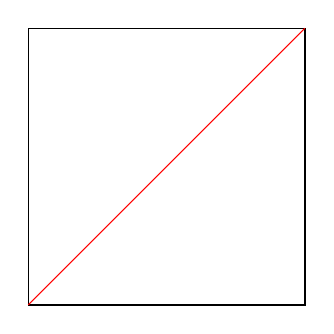
\begin{tikzpicture}
\draw [fill=white,fill opacity=0.5] (0,0)--(0,100pt)--(100pt,100pt)--(100pt,0)--(0,0);
\draw [fill=red,fill opacity=0.5,draw=red] (0,0)--(100pt,100pt);
\end{tikzpicture}
\end{figure}

احتمال اینکه این دو نقطه در دو طرف متفاوت قطر مربع انتخاب شوند و فاصله‌ی هر یک از آنها از قطر نشان داده شده‌ی مربع (قطر قرمز رنگ در شکل) بیش از 0.5 باشد چقدر است؟

%%%%%%%%%%%%%%%%%%%%%%%%%%%%%%%%%%%%%%

\Q
دو جعبه در اختیار داریم. جعبه 1 شامل 10 توپ سفید و 10 توپ آبی و جعبه دوم شامل 20 توپ سفید و 30 توپ قرمز است. ابتدا یکی از جعبه ها را به تصادف انتخاب کرده و سپس از داخل جعبه انتخاب شده، گلوله ای را به تصادف بر می داریم. 

الف) اگر گلوله سفید باشد، با چه احتمالی از جعبه‌ی 2 انتخاب شده است؟

ب) اگر گلوله سفید نباشد، با چه احتمالی قرمز است؟

%%%%%%%%%%%%%%%%%%%%%%%%%%%%%%%%%%%%%%

\Q
یک تاس سالم (که احتمال رخداد هر وجه آن $\frac{1}{6}$ است) را دوبار پرتاب می‌کنیم و نتیجه دوبار پرتاب را در نظر می‌گیریم. اگر واقعه‌ی $A$ معادل حالت هایی باشد که مجموع دو عدد رو آمده کمتر از 5 باشد، و واقعه‌ی $B$ به گونه‌ای باشد که 
$$B=\{(1,4),(2,3),(2,2),(1,2),(3,1)\},$$
در این صورت مقدار احتمال $P(A-B)$ را با بهره گیری از تعریف اصل موضوعی احتمال (کولموگروف) بیابید.

%%%%%%%%%%%%%%%%%%%%%%%%%%%%%%%%%%%%%%

\Q
یک سکه سالم را می اندازیم. اگر رو آمد، تاس سالمی را می اندازیم و عدد رو آمده را یادداشت می‌کنیم و در غیر این صورت، سه تاس را پرتاب کرده و مجموع سه عدد را یادداشت می کنیم. با چه احتمالی، عدد یادداشت شده برابر 4 است؟

%%%%%%%%%%%%%%%%%%%%%%%%%%%%%%%%%%%%%%

\Q
از مجموعه‌ی تمام اعداد دو رقمی بدون ارقام تکراری ای که می‌توان از ارقام 1، 5، 7 و 9 ساخت، عددی را به تصادف بر می گزینیم. با چه احتمالی عدد انتخاب شده، بر 3 بخش پذیر است؟

%%%%%%%%%%%%%%%%%%%%%%%%%%%%%%%%%%%%%%

\Q
کشوری شامل دو استان 1 و 2 است. استان 1 ، شامل 60 مرد و 40 زن و استان 2 شامل 650 زن و 350 مرد است. در استان 1 ، 10 مرد و 10 زن چشم آبی و در استان 2 ، 30 مرد و 20 زن چشم آبی هستند. فردی را به تصادف از این کشور انتخاب می‌کنیم.

الف) اگر این فرد چشم آبی باشد، با چه احتمالی از استان 1 انتخاب شده است؟

ب) اگر این فرد زن باشد، با چه احتمالی از استان 2 انتخاب شده و چشم آبی نیست؟

پ) اگر فرد انتخاب شده مرد باشد، با چه احتمالی چشم آبی است؟

%%%%%%%%%%%%%%%%%%%%%%%%%%%%%%%%%%%%%%

\Q
استانی دارای دو شهر است. شهر 1 دارای 120 مرد و 80 زن و شهر 2 دارای 1000 زن و 800 مرد است. در شهر 1،  50 مرد و 30 زن و در شهر 2، 100 مرد و 150 زن به تب کریمه کنگو مبتلا هستد. فردی را از این استان به تصادف انتخاب می‌کنیم.

الف) با چه احتمالی این فرد، زن سالمی از شهر 1 است؟

ب) اگر فردی که انتخاب می‌کنیم بیمار باشد، با چه احتمالی مردی از شهر 2 است؟

پ) اگر فرد انتخاب شده سالم باشد، احتمال زن بودن او چقدر است؟

%%%%%%%%%%%%%%%%%%%%%%%%%%%%%%%%%%%%%%

\Q
یک سکه سالم را برداشته، آن را سه بار پرتاب می کنیم و نتیجه‌ی سه بار پرتاب را در نظر می‌گیریم. اگر رو آمدن سکه را با H و پشت آمدن را با T نمایش دهیم:

الف) فضای نمونه را بیابید.

ب) این مسئله‌ی احتمال، چند واقعه‌ی محتمل دارد؟ (واقعه طبق تعریف یک زیر مجموعه از فضای نمونه است).

پ) طبق تعریف کلاسیک احتمال، واقعه‌ی اینکه در پرتاب اول و دوم سکه نتیجه یکسان باشد (در پرتاب سوم نتیجه دلخواه است)، با چه احتمالی رخ می دهد؟

%%%%%%%%%%%%%%%%%%%%%%%%%%%%%%%%%%%%%%

\Q
دو مجموعه‌ی 
$A=\{1,4,5\}$
و
$B=\{2,3,4\}$
 را در نظر بگیرید. مجموعه های زیر را به دست آورید.

الف) $A\cap B$
\quad,\quad
ب) $A-B$
\quad,\quad
پ) $A\times B$ (ضرب دکارتی)

ت) اگر 
$C=\{2,5,6\}$
، با محاسبه‌ی مجموعه های 
$(A\cup B)\cap C$
و
$(A\cap C)\cup (B\cap C)$
نشان دهید
$
(A\cup B)\cap C=(A\cap C)\cup (B\cap C)
$.

%%%%%%%%%%%%%%%%%%%%%%%%%%%%%%%%%%%%%%

\Q
به کمک تعریف اصولی احتمال (و با بهره گیری از اصول کولموگروف)، برای هر دو مجموعه‌ی A و B نتیجه بگیرید
$
P(A)=P(A-B)+P(A\cap B)
$.

%%%%%%%%%%%%%%%%%%%%%%%%%%%%%%%%%%%%%%

\Q
در یک کیسه، 5 گلوله‌ی آبی و 3 گلوله‌ی سفید وجود دارد. دو عدد گلوله بر می‌داریم. احتمال این را که یکی از گلوله ها آبی و دیگری سفید باشد، در دو حالت با جایگذاری و بدون جایگذاری به دست آورید (جایگذاری حالتی است که گلوله ای را پس از بیرون آوردن از کیسه و مشاهده‌ی رنگ آن، به کیسه باز گردانیم).

%%%%%%%%%%%%%%%%%%%%%%%%%%%%%%%%%%%%%%

\Q
در نقشه‌ی زیر، از شهر $A$ به شهر $B$ دو مسیر و از $B$ به $C$ یا از $A$ به $C$ یک مسیر وجود دارد. اگر احتمال قطع شدن هر مسیر مستقل از سایرین برابر $p$ باشد، احتمال آن که شخصی بتواند از شهر $A$ به $C$ برود چقدر است؟
\pic{Q2.pdf}{100mm}

%%%%%%%%%%%%%%%%%%%%%%%%%%%%%%%%%%%%%%

\Q
در مبحث مدولاسیون دیجیتال، می‌توان هر سمبل مخابراتی را با تعدادی بیت کد نموده و پس از شکل دهی پالس روی کانال ارسال کرد. فرض کنید یک سمبل مخابراتی از $n$ بیت تشکیل شده باشد. به طور مثال
\eqn{
S_k\equiv (1010001101)_2
}{}
که $k$ اندیس سمبل است و در اینجا سمبل از $10$ بیت تشکیل شده است. این سمبل از یک کانال مخابراتی ارسال و در انتهای کانال دریافت می‌شود. اگر احتمال خرابی هر بیت مستقل از سایرین برابر $p$ باشد، با چه احتمالی سمبل به درستی آشکار \underline{نمی‌شود}؟

%%%%%%%%%%%%%%%%%%%%%%%%%%%%%%%%%%%%%%

\Q
دو تاس را پرتاب می‌کنیم. احتمال اینکه دو عدد رو آمده نسبت به هم اول باشند چقدر است؟

%%%%%%%%%%%%%%%%%%%%%%%%%%%%%%%%%%%%%%

\Q
یک سکه‌ی سالم و یک تاس سالم را با هم پرتاب می کنیم.

الف) احتمال اینکه سکه به رو بیفتد و تاس عدد فرد شود را به دست آورید.

ب) احتمال اینکه سکه به رو بیفتد یا تاس عدد فرد شود را به دست آورید (هر دو باهم نیز می‌توانند رخ دهند!)

%%%%%%%%%%%%%%%%%%%%%%%%%%%%%%%%%%%%%%

\Q
یک تاس را پرتاب می کنیم. اگر مضرب 3 ظاهر شد، نتیجه را یادداشت می کنیم و در غیر این صورت سکه ای را می اندازیم و نتیجه‌ی سکه (پشت یا رو) را می نویسیم.

الف) فضای شدنی این مسئله را بیابید.

ب) با چه احتمالی واقعه‌ی رو آمدن سکه رخ می‌دهد؟

پ) احتمال واقعه‌ی اینکه تاس عدد 1 بیاید یا سکه به پشت ظاهر شود را به دست آورید.

%%%%%%%%%%%%%%%%%%%%%%%%%%%%%%%%%%%%%%

\Q
نقطه‌ای را از داخل مربع زیر بر می‌گزینیم (طول ضلع مربع برابر 2 است).

\begin{figure}[h!]
\centering
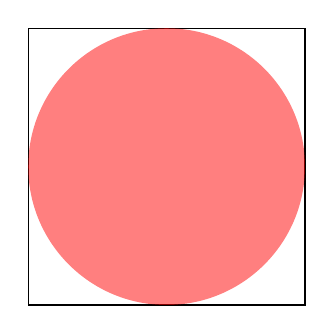
\begin{tikzpicture}
\draw [fill=white,fill opacity=0.5] (0,0)--(0,100pt)--(100pt,100pt)--(100pt,0)--(0,0);
\node [circle,minimum size=100pt,fill=red,fill opacity=0.5] (1) at(50pt,50pt) {};
\end{tikzpicture}
\end{figure}

احتمال اینکه،

الف) نقطه داخل دایره‌ی واحد (نشان داده شده در شکل) بیفتد چقدر است؟

ب) نقطه روی یکی از دو قطر مربع بیفتد چقدر است؟

پ) فاصله‌ی نقطه از هر یک از رأس های مربع بیش از $0.5$ باشد چقدر است؟

%%%%%%%%%%%%%%%%%%%%%%%%%%%%%%%%%%%%%%

\Q
از بین اعداد سه رقمی‌ای که با ترکیب رقم های 0، 1 و  2 می‌توان ساخت (تکرار مجاز است):

الف) چند عدد به 3 بخش پذیرند؟

ب) اگر عددی را به تصادف برگزینیم، با چه احتمالی زوج خواهد بود؟

%%%%%%%%%%%%%%%%%%%%%%%%%%%%%%%%%%%%%%

\Q
در یک جامعه‌ی آماری، نسبت جمعیت زنان بزرگسال، مردان بزرگسال و کودکان به کل جمعیت جامعه به ترتیب برابر $0.37$، $0.43$ و $0.2$ است. در این جامعه، $0.15$ مردان بزرگسال و $0.25$ زنان بزرگسال به نوعی بیماری مبتلا شده اند. فرد بزرگسالی را به تصادف از این جامعه انتخاب می‌کنیم، احتمال بیمار بودن او چقدر است؟

%%%%%%%%%%%%%%%%%%%%%%%%%%%%%%%%%%%%%%

\Q
فرض کنید مجموعه های B و C مستقل و دارای احتمال مثبت باشند. در چه حالتی داریم
$
P(A|B\cap C)=P(A|B)P(A|C)
$
؟

%%%%%%%%%%%%%%%%%%%%%%%%%%%%%%%%%%%%%%

\Q
(کران پایین برای احتمال اجتماع) برای هر دو مجموعه‌ی A و B ثابت کنید
$$
P(A)+P(B)-\frac{1}{4\max\{1-P(A),1-P(B)\}}
\le 
P(A\cup B).
$$

%%%%%%%%%%%%%%%%%%%%%%%%%%%%%%%%%%%%%%

\Q
جعبه‌ی 1 حاوی 1000 لامپ است که 10 درصد آنها خراب هستند. جعبه‌ی 2 نیز حاوی 2000 لامپ است که 5 درصد آنها خراب هستند. از یک جعبه که به طور تصادفی انتخاب شده، دو لامپ بیرون آورده می شوند.

الف) احتمال خرابی هر دو چقدر است؟

ب) اگر هر دو لامپ خراب باشند، با چه احتمالی جعبه‌ی 1 انتخاب شده است؟

%%%%%%%%%%%%%%%%%%%%%%%%%%%%%%%%%%%%%%

\Q
نشان دهید که برای استقلال $n$ رخداد باید 
$2^n-n-1$
 معادله برقرار باشد.

%%%%%%%%%%%%%%%%%%%%%%%%%%%%%%%%%%%%%%

\Q
در یک گل فروشی، 10 گل لاله، 5 نسترن، 3 بنفشه، 2 اقاقیا و 1 رز هلندی وجود دارد. می‌خواهیم دسته گلی شامل 5 گل که همگی به تصادف انتخاب شده باشند، برگزینیم. با چه احتمالی

الف) دسته گل شامل 2 نسترن و 2 بنفشه است؟

ب) دسته گل شامل هیچ گل لاله و بنفشه ای نیست؟

پ) دسته گل شامل حداقل یک گل از هر یک از 4 نوع گل است؟

ت) تمام گلها، از نظر نوع متمایزند؟

(دقت کنید گل های هر نوع با هم فرقی نمی کنند!)

%%%%%%%%%%%%%%%%%%%%%%%%%%%%%%%%%%%%%%

\Q
الف) از یک مجموعه‌ی $n$ عضوي، یک زیر مجموعه به تصادف انتخاب می کنیم. احتمال آن که این زیر مجموعه $k$ عضوي باشد چقدر است؟

ب) به کمک قسمت قبل ثابت کنید
$
\sum_{k=0}^n\binom{n}{k}=2^n
$.

%%%%%%%%%%%%%%%%%%%%%%%%%%%%%%%%%%%%%%

\Q
احتمال اینکه فردی به
\lr{covid-19}
 مبتلا شود، در صورتی که ماسک نزند برابر $70\%$ و در صورتی که ماسک بزند برابر $15\%$ است. اگر این فرد به طور متوسط $5\%$ مواقع ماسک بزند، احتمال کرونا گرفتن او چقدر است؟

%%%%%%%%%%%%%%%%%%%%%%%%%%%%%%%%%%%%%%

\Q
دو تاس می اندازیم و جمع دو عدد رو آمده را یادداشت می کنیم.

الف) احتمال اینکه عدد رو آمده، زوج باشد چقدر است؟

ب) اگر جمع دو عدد رو آمده زوج باشد، با چه احتمالی بیشتر از 8 است؟

%%%%%%%%%%%%%%%%%%%%%%%%%%%%%%%%%%%%%%

\Q
از بین $2^n$ زیرمجموعه‌ی مجموعه‌ی $S=\{1,2,\cdots,n\}$، دو زیر مجموعه به تصادف و مستقل از هم بر می داریم. اگر این دو زیر مجموعه، دارای اشتراک $\{1,2\}$ باشند، احتمال آن که یکی از زیرمجموعه‌ها شامل عضوهای 3، 4 و 5 باشد چقدر است؟ ($n\ge 5$)

%%%%%%%%%%%%%%%%%%%%%%%%%%%%%%%%%%%%%%

\Q
سه جعبه در اختیار داریم. در جعبه‌ی 1، 1000 لامپ موجود است که 3تای آنها معیوبند. جعبه‌ی 2 شامل 10 لامپ است که 3 تای آنها معیوبند و در جعبه‌ی سوم هم 3000 لامپ وجود دارد که همگی سالمند. اگر یکی از این جعبه ها را به تصادف برگزیده و از داخل آن لامپی انتخاب کنیم،

الف) با چه احتمالی لامپ معیوب است؟

ب) اگر لامپ معیوب باشد، با چه احتمالی از جعبه‌ی 2 انتخاب شده است؟

پ) اگر لامپ سالم باشد، با چه احتمالی از یکی از جعبه‌های 1 یا 2 انتخاب شده است؟

%%%%%%%%%%%%%%%%%%%%%%%%%%%%%%%%%%%%%%



\Q
از یک جعبه که دارای $M$ گلوله‌ی سفید و $N-M$ گلوله‌ی سیاه است، $n$ گلوله برداشته می‌شود.

الف)
احتمال آنکه $m$ گلوله از گلوله های برداشته شده سفید باشند در حالت با جایگذاری چقدر است؟

ب)
احتمال آنکه $m$ گلوله از گلوله های برداشته شده سفید باشند در حالت بدون جایگذاری چقدر است؟

ج) اگر بدانیم تمام گلوله های سفید برداشته شده اند، احتمال آنکه دقیقا 2 گلوله‌ی سیاه نیز برداشته شده باشند چقدر است؟

%%%%%%%%%%%%%%%%%%%%%%%%%%%%%%%%%%%%%%

\Q
سکه ای را پرتاب می‌کنیم. اگر رو آمد، دو تاس را پرتاب کرده، جمع دو عدد روی تاس را یادداشت می کنیم. اگر سکه پشت آمد، یک تاس را پرتاب کرده و عدد آنرا یادداشت می کنیم. با چه احتمالی

الف) عدد یادداشت شده برابر 3 است؟
\quad,\quad
ب) عدد یادداشت شده برابر 8 است؟

%%%%%%%%%%%%%%%%%%%%%%%%%%%%%%%%%%%%%%

\Q
موارد زیر را در یک مسئله‌ی احتمالاتی تعریف کنید:

الف) فضای نمونه
\quad,\quad
ب) پیشامد (واقعه)
\quad,\quad
پ) پیشامد (واقعه‌ی) ساده

%%%%%%%%%%%%%%%%%%%%%%%%%%%%%%%%%%%%%%

\Q
آیا فضای نمونه در یک مسئله‌ی احتمالاتی، تنها مجموعه با احتمال یک است؟ پاسخ را برای هر دو حالتی که فضای نمونه متناهی یا نامتناهی باشد شرح دهید و در صورت لزوم، مثال بزنید.

%%%%%%%%%%%%%%%%%%%%%%%%%%%%%%%%%%%%%%

\Q
اگر $A$ فضای نمونه‌ی آزمایش پرتاب سکه با رخدادهای پشت و رو و $B$ فضای نمونه‌ی پرتاب تاس با اعداد طبیعی 1 تا 6 باشد،

الف) حاصلضرب دکارتی $A$ و $B$ (
$A\times B$
)
را به دست آورید. این مجموعه، فضای نمونه‌ی چه آزمایشی است؟

ب) دو زیر مجموعه‌ی 3 عضوی از مجموعه‌ی 
$
A\times B
$
برگزینید که با یکدیگر ناسازگار باشند. آیا می‌توانید همین کار را برای زیرمجموعه‌های 7 عضوی تکرار کنید؟ چرا؟

%%%%%%%%%%%%%%%%%%%%%%%%%%%%%%%%%%%%%%

\Q
با بهره گیری از جبر مجموعه ها و اصول کولموگروف احتمال، نشان دهید اگر $A$، $B$ و $C$ سه مجموعه‌ باشند به طوری که 
$
P(B\cap C)=0
$
، در این صورت
$$
P\left\{
A\cap(B\cup C)
\right\}
=
P\left\{
A\cap B
\right\}
+
P\left\{
A\cap C
\right\}
.
$$

%%%%%%%%%%%%%%%%%%%%%%%%%%%%%%%%%%%%%%

\Q
در یک جامعه، احتمال اینکه فردی به کرونا مبتلا باشد $0.07$ و احتمال آن که به آنفلوآنزا مبتلا باشد $0.19$ است. اگر 20 درصد افراد این جامعه مبتلا به حداقل یکی از این دو بیماری باشند،

الف) چند درصد افراد به هر دو بیماری مبتلا هستند؟

ب) چند درصد افراد \underline{فقط} به کرونا مبتلا هستند؟

%%%%%%%%%%%%%%%%%%%%%%%%%%%%%%%%%%%%%%

\Q
یک عدد از مجموعه‌ی 
$
\{1,2,3,\cdots,10\}
$
به تصادف بر می‌گزینیم. اگر تمام وقایع ساده هم شانس باشند و تعریف کنیم
$
A=\{2,3,5,7\}
$
و
$
B=\{1,3,5,7,9\}
$،

الف) مقدار
$P(A)$
را بیابید.

ب) مجموعه‌های 
$A-B$
و
$A\cap B$
را به دست آورده و مقادیر 
$P(A-B)$
و
$P(A\cap B)$
را بیابید.

پ) تحقیق کنید
$
P(A-B)=P(A)-P(A\cap B)
$.
چه توجیهی برای پاسخ شما وجود دارد؟

%%%%%%%%%%%%%%%%%%%%%%%%%%%%%%%%%%%%%%

\Q
در یک کتابخانه، سه کتاب فیزیک، دو کتاب رمان و چهار کتاب روان شناسی موجود است. مطلوبست تعداد حالات چیدن این کتاب ها در یک قفسه کنار هم چنانچه:

الف) تمام کتابهای هم نوع متمایز باشند (مثلا ترتیب دو کتاب رمان نسبت به هم مهم باشد).

ب) تمام کتابهای هم نوع نامتمایز باشند (مثلا ترتیب دو کتاب رمان نسبت به هم مهم نباشد).

%%%%%%%%%%%%%%%%%%%%%%%%%%%%%%%%%%%%%%

\Q
اعضای یک شرکت شامل 1 مدیرعامل، 2 منشی، 1 حسابدار و 5 نفر از سایر اعضای هیئت مدیره در یک میزگرد دارای 11 صندلی می‌نشینند. مطلوبست تعداد حالاتی که

الف) هر دو منشی کنار هم باشند.

ب) هیچ یک از اعضای هیئت مدیره (به جز مدیرعامل)، مجاور مدیرعامل نباشد.

پ) حسابدار کنار مدیرعامل بنشیند و تمام اعضای هیئت مدیره (به جز مدیرعامل) کنار هم باشند.

(راهنمایی: برای حل این سوال، به تمایز یا عدم تمایز اعضای هیئت مدیره یا منشی ها دقت کنید. آیا منطقی است متمایز باشند یا نباشند؟ همچنین دقت کنید که همواره دو صندلی از میزگرد خالی می مانند و باید در شمارش حالات محاسبه شوند.)

%%%%%%%%%%%%%%%%%%%%%%%%%%%%%%%%%%%%%%

\Q
در کیسه ای، 10 توپ آبی و 7 توپ قرمز موجود است. دو توپ به تصادف و بدون جایگذاری بر می‌داریم.

الف) اگر توپهای همرنگ نامتمایز باشند، تعداد حالات برداشتن دو توپ غیرهمرنگ چقدر است؟

ب) اگر توپهای همرنگ نامتمایز باشند، احتمال برداشتن دو توپ غیرهمرنگ چقدر است؟

پ) اگر توپهای آبی را از 1 تا 10 و توپهای قرمز را از 1 تا 7 شماره گذاری کنیم، احتمال آنکه توپ آبی شماره 4 و توپ آبی شماره 3 برداشته شود چقدر است؟

ت) اگر توپهای آبی را از 1 تا 10 و توپهای قرمز را از 1 تا 7 شماره گذاری کنیم، آیا احتمال برداشتن دو توپ غیرهمرنگ، با مقدار بدست آمده در قسمت الف تفاوت می‌کند؟ توضیح دهید.

%%%%%%%%%%%%%%%%%%%%%%%%%%%%%%%%%%%%%%

\Q
قسمتهای ب)، پ) و ت) مسئله‌ی پیش را با فرض داشتن جایگذاری حل کنید؛ یعنی زمانی که توپ اول را برداشتیم، رنگ آن را یادداشت کرده، آنرا به کیسه بازگردانده و سپس توپ دوم را بر می‌داریم.

%%%%%%%%%%%%%%%%%%%%%%%%%%%%%%%%%%%%%%

\Q
نقطه‌ای را از داخل مربع به تصادف انتخاب می‌کنیم. احتمال آنکه فاصله‌ی این نقطه تا مرکز مربع، از فاصله‌ی این نقطه تا هر یک از رئوس مربع بیشتر باشد چقدر است؟

%%%%%%%%%%%%%%%%%%%%%%%%%%%%%%%%%%%%%%

\Q
از مجموعه‌ی زیرمجموعه‌های مجموعه‌ی
$
\{1,2,3,\cdots,n\}
$
، دو زیرمجموعه‌‌‌ی متمایز به تصادف انتخاب می‌کنیم. با چه احتمالی، این دو زیرمجموعه ناسازگارند؟

%%%%%%%%%%%%%%%%%%%%%%%%%%%%%%%%%%%%%%

\Q
الف) در یک صفحه‌ی شطرنجی 8 در 8، یک مهره‌ی رخ سفید به تصادف در یکی از خانه‌های این صفحه قرار می‌گیرد. سپس، یک مهره‌ی رخ سیاه را به تصادف در یکی از خانه‌های این صفحه قرار می‌دهیم. با چه احتمالی، رخ سیاه در معرض حمله‌ی رخ سفید قرار می‌گیرد؟ (حرکت رخ، به صورت افقی یا عمودی در صفحه است)

ب) یک مهره‌ی شاه سفید، در یکی از گوشه‌های یک صفحه‌ی شطرنجی 8 در 8 قرار دارد. دو رخ سیاه به تصادف در دو خانه‌ی این صفحه قرار می‌گیرند. با چه احتمالی، شاه سفید مات می‌شود؟ (مات شدن شاه، زمانی اتفاق می‌افتد که نوبت حرکت شاه بوده و با هر حرکت، در معرض حمله‌ی یکی از مهره‌های دشمن قرار گیرد)

\begin{figure}[h]
\centering

\begin{tikzpicture}
\filldraw[fill=black](-3.2,-3.2)--(-2.4000000000000004,-3.2)--(-2.4000000000000004,-2.4000000000000004)--(-3.2,-2.4000000000000004)--(-3.2,-3.2);
\filldraw[fill=white](-3.2,-2.4000000000000004)--(-2.4000000000000004,-2.4000000000000004)--(-2.4000000000000004,-1.6000000000000003)--(-3.2,-1.6000000000000003)--(-3.2,-2.4000000000000004);
\filldraw[fill=black](-3.2,-1.6)--(-2.4000000000000004,-1.6)--(-2.4000000000000004,-0.8)--(-3.2,-0.8)--(-3.2,-1.6);
\filldraw[fill=white](-3.2,-0.8)--(-2.4000000000000004,-0.8)--(-2.4000000000000004,0.0)--(-3.2,0.0)--(-3.2,-0.8);
\filldraw[fill=black](-3.2,0.0)--(-2.4000000000000004,0.0)--(-2.4000000000000004,0.8)--(-3.2,0.8)--(-3.2,0.0);
\filldraw[fill=white](-3.2,0.8)--(-2.4000000000000004,0.8)--(-2.4000000000000004,1.6)--(-3.2,1.6)--(-3.2,0.8);
\filldraw[fill=black](-3.2,1.6)--(-2.4000000000000004,1.6)--(-2.4000000000000004,2.4000000000000004)--(-3.2,2.4000000000000004)--(-3.2,1.6);
\filldraw[fill=white](-3.2,2.4000000000000004)--(-2.4000000000000004,2.4000000000000004)--(-2.4000000000000004,3.2)--(-3.2,3.2)--(-3.2,2.4000000000000004);
\filldraw[fill=white](-2.4000000000000004,-3.2)--(-1.6000000000000003,-3.2)--(-1.6000000000000003,-2.4000000000000004)--(-2.4000000000000004,-2.4000000000000004)--(-2.4000000000000004,-3.2);
\filldraw[fill=black](-2.4000000000000004,-2.4000000000000004)--(-1.6000000000000003,-2.4000000000000004)--(-1.6000000000000003,-1.6000000000000003)--(-2.4000000000000004,-1.6000000000000003)--(-2.4000000000000004,-2.4000000000000004);
\filldraw[fill=white](-2.4000000000000004,-1.6)--(-1.6000000000000003,-1.6)--(-1.6000000000000003,-0.8)--(-2.4000000000000004,-0.8)--(-2.4000000000000004,-1.6);
\filldraw[fill=black](-2.4000000000000004,-0.8)--(-1.6000000000000003,-0.8)--(-1.6000000000000003,0.0)--(-2.4000000000000004,0.0)--(-2.4000000000000004,-0.8);
\filldraw[fill=white](-2.4000000000000004,0.0)--(-1.6000000000000003,0.0)--(-1.6000000000000003,0.8)--(-2.4000000000000004,0.8)--(-2.4000000000000004,0.0);
\filldraw[fill=black](-2.4000000000000004,0.8)--(-1.6000000000000003,0.8)--(-1.6000000000000003,1.6)--(-2.4000000000000004,1.6)--(-2.4000000000000004,0.8);
\filldraw[fill=white](-2.4000000000000004,1.6)--(-1.6000000000000003,1.6)--(-1.6000000000000003,2.4000000000000004)--(-2.4000000000000004,2.4000000000000004)--(-2.4000000000000004,1.6);
\filldraw[fill=black](-2.4000000000000004,2.4000000000000004)--(-1.6000000000000003,2.4000000000000004)--(-1.6000000000000003,3.2)--(-2.4000000000000004,3.2)--(-2.4000000000000004,2.4000000000000004);
\filldraw[fill=black](-1.6,-3.2)--(-0.8,-3.2)--(-0.8,-2.4000000000000004)--(-1.6,-2.4000000000000004)--(-1.6,-3.2);
\filldraw[fill=white](-1.6,-2.4000000000000004)--(-0.8,-2.4000000000000004)--(-0.8,-1.6000000000000003)--(-1.6,-1.6000000000000003)--(-1.6,-2.4000000000000004);
\filldraw[fill=black](-1.6,-1.6)--(-0.8,-1.6)--(-0.8,-0.8)--(-1.6,-0.8)--(-1.6,-1.6);
\filldraw[fill=white](-1.6,-0.8)--(-0.8,-0.8)--(-0.8,0.0)--(-1.6,0.0)--(-1.6,-0.8);
\filldraw[fill=black](-1.6,0.0)--(-0.8,0.0)--(-0.8,0.8)--(-1.6,0.8)--(-1.6,0.0);
\filldraw[fill=white](-1.6,0.8)--(-0.8,0.8)--(-0.8,1.6)--(-1.6,1.6)--(-1.6,0.8);
\filldraw[fill=black](-1.6,1.6)--(-0.8,1.6)--(-0.8,2.4000000000000004)--(-1.6,2.4000000000000004)--(-1.6,1.6);
\filldraw[fill=white](-1.6,2.4000000000000004)--(-0.8,2.4000000000000004)--(-0.8,3.2)--(-1.6,3.2)--(-1.6,2.4000000000000004);
\filldraw[fill=white](-0.8,-3.2)--(0.0,-3.2)--(0.0,-2.4000000000000004)--(-0.8,-2.4000000000000004)--(-0.8,-3.2);
\filldraw[fill=black](-0.8,-2.4000000000000004)--(0.0,-2.4000000000000004)--(0.0,-1.6000000000000003)--(-0.8,-1.6000000000000003)--(-0.8,-2.4000000000000004);
\filldraw[fill=white](-0.8,-1.6)--(0.0,-1.6)--(0.0,-0.8)--(-0.8,-0.8)--(-0.8,-1.6);
\filldraw[fill=black](-0.8,-0.8)--(0.0,-0.8)--(0.0,0.0)--(-0.8,0.0)--(-0.8,-0.8);
\filldraw[fill=white](-0.8,0.0)--(0.0,0.0)--(0.0,0.8)--(-0.8,0.8)--(-0.8,0.0);
\filldraw[fill=black](-0.8,0.8)--(0.0,0.8)--(0.0,1.6)--(-0.8,1.6)--(-0.8,0.8);
\filldraw[fill=white](-0.8,1.6)--(0.0,1.6)--(0.0,2.4000000000000004)--(-0.8,2.4000000000000004)--(-0.8,1.6);
\filldraw[fill=black](-0.8,2.4000000000000004)--(0.0,2.4000000000000004)--(0.0,3.2)--(-0.8,3.2)--(-0.8,2.4000000000000004);
\filldraw[fill=black](0.0,-3.2)--(0.8,-3.2)--(0.8,-2.4000000000000004)--(0.0,-2.4000000000000004)--(0.0,-3.2);
\filldraw[fill=white](0.0,-2.4000000000000004)--(0.8,-2.4000000000000004)--(0.8,-1.6000000000000003)--(0.0,-1.6000000000000003)--(0.0,-2.4000000000000004);
\filldraw[fill=black](0.0,-1.6)--(0.8,-1.6)--(0.8,-0.8)--(0.0,-0.8)--(0.0,-1.6);
\filldraw[fill=white](0.0,-0.8)--(0.8,-0.8)--(0.8,0.0)--(0.0,0.0)--(0.0,-0.8);
\filldraw[fill=black](0.0,0.0)--(0.8,0.0)--(0.8,0.8)--(0.0,0.8)--(0.0,0.0);
\filldraw[fill=white](0.0,0.8)--(0.8,0.8)--(0.8,1.6)--(0.0,1.6)--(0.0,0.8);
\filldraw[fill=black](0.0,1.6)--(0.8,1.6)--(0.8,2.4000000000000004)--(0.0,2.4000000000000004)--(0.0,1.6);
\filldraw[fill=white](0.0,2.4000000000000004)--(0.8,2.4000000000000004)--(0.8,3.2)--(0.0,3.2)--(0.0,2.4000000000000004);
\filldraw[fill=white](0.8,-3.2)--(1.6,-3.2)--(1.6,-2.4000000000000004)--(0.8,-2.4000000000000004)--(0.8,-3.2);
\filldraw[fill=black](0.8,-2.4000000000000004)--(1.6,-2.4000000000000004)--(1.6,-1.6000000000000003)--(0.8,-1.6000000000000003)--(0.8,-2.4000000000000004);
\filldraw[fill=white](0.8,-1.6)--(1.6,-1.6)--(1.6,-0.8)--(0.8,-0.8)--(0.8,-1.6);
\filldraw[fill=black](0.8,-0.8)--(1.6,-0.8)--(1.6,0.0)--(0.8,0.0)--(0.8,-0.8);
\filldraw[fill=white](0.8,0.0)--(1.6,0.0)--(1.6,0.8)--(0.8,0.8)--(0.8,0.0);
\filldraw[fill=black](0.8,0.8)--(1.6,0.8)--(1.6,1.6)--(0.8,1.6)--(0.8,0.8);
\filldraw[fill=white](0.8,1.6)--(1.6,1.6)--(1.6,2.4000000000000004)--(0.8,2.4000000000000004)--(0.8,1.6);
\filldraw[fill=black](0.8,2.4000000000000004)--(1.6,2.4000000000000004)--(1.6,3.2)--(0.8,3.2)--(0.8,2.4000000000000004);
\filldraw[fill=black](1.6,-3.2)--(2.4000000000000004,-3.2)--(2.4000000000000004,-2.4000000000000004)--(1.6,-2.4000000000000004)--(1.6,-3.2);
\filldraw[fill=white](1.6,-2.4000000000000004)--(2.4000000000000004,-2.4000000000000004)--(2.4000000000000004,-1.6000000000000003)--(1.6,-1.6000000000000003)--(1.6,-2.4000000000000004);
\filldraw[fill=black](1.6,-1.6)--(2.4000000000000004,-1.6)--(2.4000000000000004,-0.8)--(1.6,-0.8)--(1.6,-1.6);
\filldraw[fill=white](1.6,-0.8)--(2.4000000000000004,-0.8)--(2.4000000000000004,0.0)--(1.6,0.0)--(1.6,-0.8);
\filldraw[fill=black](1.6,0.0)--(2.4000000000000004,0.0)--(2.4000000000000004,0.8)--(1.6,0.8)--(1.6,0.0);
\filldraw[fill=white](1.6,0.8)--(2.4000000000000004,0.8)--(2.4000000000000004,1.6)--(1.6,1.6)--(1.6,0.8);
\filldraw[fill=black](1.6,1.6)--(2.4000000000000004,1.6)--(2.4000000000000004,2.4000000000000004)--(1.6,2.4000000000000004)--(1.6,1.6);
\filldraw[fill=white](1.6,2.4000000000000004)--(2.4000000000000004,2.4000000000000004)--(2.4000000000000004,3.2)--(1.6,3.2)--(1.6,2.4000000000000004);
\filldraw[fill=white](2.4000000000000004,-3.2)--(3.2,-3.2)--(3.2,-2.4000000000000004)--(2.4000000000000004,-2.4000000000000004)--(2.4000000000000004,-3.2);
\filldraw[fill=black](2.4000000000000004,-2.4000000000000004)--(3.2,-2.4000000000000004)--(3.2,-1.6000000000000003)--(2.4000000000000004,-1.6000000000000003)--(2.4000000000000004,-2.4000000000000004);
\filldraw[fill=white](2.4000000000000004,-1.6)--(3.2,-1.6)--(3.2,-0.8)--(2.4000000000000004,-0.8)--(2.4000000000000004,-1.6);
\filldraw[fill=black](2.4000000000000004,-0.8)--(3.2,-0.8)--(3.2,0.0)--(2.4000000000000004,0.0)--(2.4000000000000004,-0.8);
\filldraw[fill=white](2.4000000000000004,0.0)--(3.2,0.0)--(3.2,0.8)--(2.4000000000000004,0.8)--(2.4000000000000004,0.0);
\filldraw[fill=black](2.4000000000000004,0.8)--(3.2,0.8)--(3.2,1.6)--(2.4000000000000004,1.6)--(2.4000000000000004,0.8);
\filldraw[fill=white](2.4000000000000004,1.6)--(3.2,1.6)--(3.2,2.4000000000000004)--(2.4000000000000004,2.4000000000000004)--(2.4000000000000004,1.6);
\filldraw[fill=black](2.4000000000000004,2.4000000000000004)--(3.2,2.4000000000000004)--(3.2,3.2)--(2.4000000000000004,3.2)--(2.4000000000000004,2.4000000000000004);
\end{tikzpicture}
\end{figure}

%%%%%%%%%%%%%%%%%%%%%%%%%%%%%%%%%%%%%%

\Q
یک سکه‌ی سالم را پرتاب می‌کنیم. اگر رو بیاید، یک تاس را پرتاب کرده و عدد روی آن را یادداشت می‌کنیم. اگر سکه پشت بیاید، دو تاس را پرتاب کرده و جمع اعداد دو تاس را یادداشت می‌کنیم. احتمال آنکه عدد رو آمده برابر $n$ باشد چقدر است؟ (
$
2\le n\le 12
$
)

%%%%%%%%%%%%%%%%%%%%%%%%%%%%%%%%%%%%%%

\Q
از کیسه‌ای که شامل 7 توپ سیاه و 10 توپ سفید است، 3 توپ به تصادف بیرون می‌آوریم. سپس از بین 3 توپ بیرون آمده، یکی را به تصادف بر می‌گزینیم. اگر بدانیم حداقل یک توپ از 3 توپ بیرون آمده سیاه است، احتمال آنکه توپ انتخابی از بین این 3 توپ، سفید باشد چقدر است؟

%%%%%%%%%%%%%%%%%%%%%%%%%%%%%%%%%%%%%%

\Q
دو کیسه در اختیار داریم. کیسه‌ی 1 شامل 7 توپ سیاه و 10 توپ سفید و کیسه‌ی 2 شامل 4 توپ سیاه، 2 توپ سفید و 3 توپ قرمز است. ابتدا یکی از کیسه‌ها را به تصادف انتخاب کرده و سپس، توپی از آن به تصادف بیرون می‌آوریم. اگر بدانیم توپ انتخابی سفید نیست، با چه احتمالی از کیسه‌ی 2 انتخاب شده است؟

%%%%%%%%%%%%%%%%%%%%%%%%%%%%%%%%%%%%%%

\Q
فرض کنید در نقشه‌ی زیر قصد داریم از شهر A به شهر Z برویم. هر یک از 7 لینک نقشه‌ی زیر، با احتمال $p$ مستقل از سایر لینک ها سالم هستند. احتمال آن که مسیر سالمی از A تا Z وجود داشته باشد چقدر است؟

\begin{figure}[h]
\Large
\centering
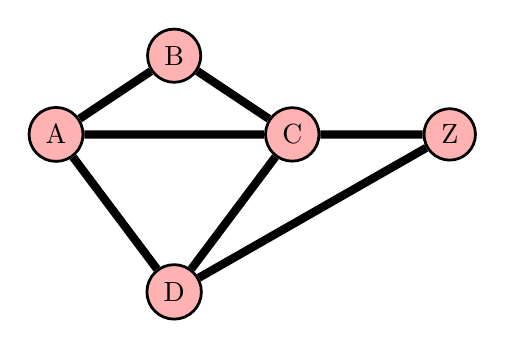
\begin{tikzpicture}
\node [draw=black,fill=white!70!red,circle,line width=1] (A) at (0,0) {A};
\node [draw=black,fill=white!70!red,circle,line width=1] (B) at (1.5,1) {B};
\node [draw=black,fill=white!70!red,circle,line width=1] (C) at (3,0) {C};
\node [draw=black,fill=white!70!red,circle,line width=1] (D) at (1.5,-2) {D};
\node [draw=black,fill=white!70!red,circle,line width=1] (Z) at (5,0) {Z};
\draw[line width=3]
(A)--(B)
(B)--(C)
(C)--(Z)
(A)--(C)
(A)--(D)
(D)--(C)
(D)--(Z)
;
\end{tikzpicture}
\end{figure}

%%%%%%%%%%%%%%%%%%%%%%%%%%%%%%%%%%%%%%

\Q
از کیسه‌ای که شامل 5 مهره سیاه، 8 مهره سفید و 1 مهره قرمز است، دو توپ به تصادف بیرون می‌آوریم. احتمال آنکه هر دو توپ همرنگ باشند چقدر است؟

%%%%%%%%%%%%%%%%%%%%%%%%%%%%%%%%%%%%%%

\Q
دو جعبه از لامپ‌ها در اختیار داریم. جعبه‌ی اول، دارای 1000 لامپ است که $1\%$ آنها سالمند. جعبه‌ی دوم، دارای 10000 لامپ است که $95\%$ آنها سالم اند. یکی از جعبه‌ها را به تصادف انتخاب کرده و دو لامپ بیرون می‌کشیم. احتمال آن که هر دو لامپ از جعبه‌ی 1 انتخاب شده باشند چقدر است اگر

الف) هر دو لامپ خراب باشند.

ب) اگر یکی از لامپ ها سالم و دیگری خراب باشد.

%%%%%%%%%%%%%%%%%%%%%%%%%%%%%%%%%%%%%%
%%%%%%%%%%%%%%%%%%%%%%%%%%%%%%%%%%%%%%
%%%%%%%%%%%%%%%%%%%%%%%%%%%%%%%%%%%%%%
%%%%%%%%%%%%%%%%%%%%%%%%%%%%%%%%%%%%%%
%%%%%%%%%%%%%%%%%%%%%%%%%%%%%%%%%%%%%%

\chapter{آزمایش های تکراری}

\Q
تاس سالمی را 3 بار پرتاب می‌کنیم و اعداد رو آمده در سه پرتاب را در نظر می‌گیریم.

الف) احتمال آن که جمع اعداد رو آمده برابر 5 باشد چقدر است؟

ب) اگر عدد رو آمده‌ی اول برابر 4 باشد، احتمال آن که جمع اعداد پرتاب ها برابر 7 باشد چقدر است؟

پ) احتمال آن که جمع اعداد تاس در پرتاب‌های فرد، برابر 5 باشد چقدر است؟

ت) احتمال آنکه از این 3 بار، حداقل 2 بار عدد زوج بیاید چقدر است؟

ث) احتمال رو آمدن مضرب 3 در پرتاب اول چقدر است؟

%%%%%%%%%%%%%%%%%%%%%%%%%%%%%%%%%%%%%%

\Q
سکه ای را پرتاب می‌کنیم. اگر رو آمد، تاسی را 3 بار پرتاب کرده و جمع اعداد رو آمده در 3 پرتاب را در نظر می‌گیریم. اگر پشت آمد، تاسی را 4 بار پرتاب کرده و جمع اعداد رو آمده در 4 پرتاب را در نظر می‌گیریم. اگر جمع اعداد روآمده‌ی تاس برابر 5 باشد، با چه احتمالی سکه پشت آمده است؟

%%%%%%%%%%%%%%%%%%%%%%%%%%%%%%%%%%%%%%

\Q
تاس سالمی را 4 بار پرتاب می کنیم و اعداد رو آمده در چهار پرتاب را در نظر می‌گیریم.

الف) اگر در دو پرتاب این تاس عدد 2 ظاهر شده باشد، احتمال آنکه در دو پرتاب دیگر عدد فردی ظاهر شده باشد چقدر است؟

ب) با چه احتمالی، جمع اعداد در پرتاب های زوج، 5 برابر جمع اعداد در پرتاب‌های فرد است؟

%%%%%%%%%%%%%%%%%%%%%%%%%%%%%%%%%%%%%%
 
\Q
سکه‌ی سالمی را 10 بار پرتاب می کنیم. مطلوبست احتمال آن که

الف) در این 10 پرتاب، حداقل دوبار رو بیاید.

ب) در سه پرتاب اول حداکثر یک بار پشت بیاید.

پ) در پرتاب های زوج، نتیجه یکسان باشد (همگی رو یا همگی پشت باشند).

الف) دقیقا 3 بار شیر بیاید.

ب) دست کم 2 بار خط بیاید.

پ) در مجموع، دقیقا 7 بار خط آمده باشد، اگر بدانیم در 5 پرتاب اول خط آمده است.

%%%%%%%%%%%%%%%%%%%%%%%%%%%%%%%%%%%%%%
 
\Q
الف) اگر یک رشته لامپ متوالی شامل $n$ لامپ که هر لامپ به احتمال $p$ خراب است، به ولتاژ برق وصل شود، با چه احتمالی روشن می شود؟ (در رشته متوالی لامپ ها، لامپ ها به صورت پشت سر هم به یکدیگر وصل شده اند.)

ب) اگر رشته لامپ موازی باشد، مسئله را حل کنید. (در رشته‌ی موازی لامپ ها، یکی از سرهای همه‌ی لامپ ها به یک نقطه و سر دیگر تمام لامپ ها به نقطه‌ی دیگر وصل شده اند.)

%%%%%%%%%%%%%%%%%%%%%%%%%%%%%%%%%%%%%%

\Q
در یک امتحان، احتمال درست پاسخ دادن به یک سوال دو گزینه ای برابر $p$ است. پس از امتحان، $n$ دانشجو پاسخ های خود را با هم مقایسه می کنند و متوجه می‌شوند که همگی به آن سوال پاسخ یکسانی داده اند. با چه احتمالی تمام این $n$ دانشجو به پاسخ درست رسیده اند؟

%%%%%%%%%%%%%%%%%%%%%%%%%%%%%%%%%%%%%%

\Q
یک سکه‌ی سالم را 7بار پرتاب می کنیم.

الف) احتمال اینکه نتیجه‌ی پرتاب اول و آخر برابر باشد چقدر است؟

ب) با چه احتمالی حداقل دو رو و سه پشت در این 7 پرتاب خواهیم داشت؟

پ) اگر نتیجه پرتاب سکه در سه پرتاب اول یکسان باشد، با چه احتمالی در این 7 پرتاب، در مجموع دقیقا 4 بار سکه رو می آید؟

%%%%%%%%%%%%%%%%%%%%%%%%%%%%%%%%%%%%%%

\Q
یک تاس سالم را 5 بار پرتاب می کنیم.

الف) اگر جمع پنج عدد رو آمده در این پنج پرتاب را در نظر بگیریم، با چه احتمالی این مجموع برابر 7 است؟

ب) با چه احتمالی عدد رو آمده در پرتاب پنجم برابر جمع اعداد رو آمده در 4 پرتاب قبلی خواهد بود؟

%%%%%%%%%%%%%%%%%%%%%%%%%%%%%%%%%%%%%%

\Q
بزرگراه 8 بانده ای را در نظر بگیرید که از هر باند آن در هر لحظه حداکثر یک ماشین می‌تواند عبور کند. اگر 9 ماشین هر یک با احتمال $p$ وارد بزرگراه شوند،

الف) با چه احتمالی همه‌ی ماشین های وارد شده به بزرگراه بدون مشکل از آن رد می‌شوند؟

ب) $p$ چقدر باشد تا احتمال قسمت الف بیشتر از $0.99$ باشد؟

%%%%%%%%%%%%%%%%%%%%%%%%%%%%%%%%%%%%%%

\Q
دو تیم ورزشی A و B در یک بازی در 9 دست با هم روبرو می‌شوند و نتیجه‌ی هر دست فقط برد یکی از دو تیم می‌تواند باشد. فرض کنید تیم A با احتمال $p$ در هر دست پیروز می‌شود و نتیجه‌ی دست‌ها مستقل از هم است. برنده‌ی بازی کسی است که بیشتر بازی ها را برده باشد.

الف) با چه احتمالی تیم A پس از 6 دست موفق به بردن بازی می‌شود؟

ب) اگر بدانیم تیم A در نهایت بازی را برده است، با چه احتمالی در حداقل یک دست به تیم B باخته است؟

ج) به ازای $p=0.5$، اگر بدانیم تیم A دست اول را برده، با چه احتمالی بازی را می‌برد؟

%%%%%%%%%%%%%%%%%%%%%%%%%%%%%%%%%%%%%%

\Q
یک سکه‌ی سالم $n$ بار پرتاب شده و $k$ بار رو آمده است. کوچکترین مقدار $n$ را بیابید به گونه‌ای که
$$
P\left\{0.49\le{k\over n}\le0.51\right\}>0.95
$$

%%%%%%%%%%%%%%%%%%%%%%%%%%%%%%%%%%%%%%

\Q
قضیه‌ی دموآو-لاپلاس در چه حالتی برای تکرر توزیع برنولی به تعداد $n$ بار برقرار است؟ به کمک یک ماشین حساب یا کامپیوتر، مقادیر 
$\binom{n}{k}p^k(1-p)^{n-k}$
و
$e^{-np}{(np)^k\over k!}$
 را به ازای حالت های مختلف 
$n$
و
$p$
محاسبه کرده و خطای تقریب پواسون را به دست آورید.

الف)
$n=10\quad,\quad p=0.7\quad,\quad k=7$

ب)
$n=30\quad,\quad p=0.3\quad,\quad k=9$

پ)
$n=50\quad,\quad p=0.02\quad,\quad k=1$

ت)
$n=300\quad,\quad p=0.01\quad,\quad k=3$

ث)
$n=30\quad,\quad p=0.8\quad,\quad k=24$

ج)
$n=1000\quad,\quad p=0.5\quad,\quad k=1$

چ)
$n=1000\quad,\quad p=0.5\quad,\quad k=300$

ح)
$n=1000\quad,\quad p=0.5\quad,\quad k=490$

در کدام حالت تقریب پواسون، خطای کمتری دارد و چرا؟

%%%%%%%%%%%%%%%%%%%%%%%%%%%%%%%%%%%%%%

\Q
سکه‌ای را پرتاب می‌کنیم. اگر پشت آمد، آن را 9 بار دیگر پرتاب می‌کنیم و نتایج 10 پرتاب را در نظر می‌گیریم. اگر رو آمد، آن را 5 بار دیگر پرتاب می‌کنیم و نتایج 6 پرتاب را در نظر می‌گیریم. احتمال آن که در تمام پرتاب های سکه، دقیقأ 6 بار رو بیاید چقدر است؟

%%%%%%%%%%%%%%%%%%%%%%%%%%%%%%%%%%%%%%

\Q
یک آزمایش برنولی را که احتمال موفقیت در آن برابر 
$
40\%
$
است، $n$ بار تکرار می‌کنیم. اگر $k$، برابر تعداد موفقیت‌ها در این پرتاب ها باشد، $n$ حداقل چقدر باشد تا احتمال رخداد 
$
\{38\%<\frac{k}{n}<42\%\}
$
بیش از 
$
70\%
$
باشد؟

(راهنمایی: از قضیه‌ی دموآور-لاپلاس استفاده نمایید.)

(جدول مربوط به محاسبه‌ی تابع 
$
G^{-1}(x)
$
در صفحه‌ی بعد آمده است.
)

\newpage

%\newgeometry{left=0mm,right=0mm}

%\begin{figure}[h]
%\centering
%\includegraphics[width=220mm]{ginv.pdf}
%\end{figure}

%(تنها نامساوی مربوط به قضیه‌ی دموآور-لاپلاس را نوشته، اعداد را جایگذاری نموده و ساده کنید. محاسبه‌ی دقیق مقدار $n$ الزامی نیست.)
%سکه‌ای را پرتاب می‌کنیم. اگر رو آمد، یک تاس سالم را 5 بار پرتاب کرده و جمع اعداد این 5 پرتاب را می‌نویسیم.

\begin{table}[h]
\centering
\large
\lr{
\begin{tabular}{|c|c|c|c|c|c|c|c|}
\hline
$x$&$G^{-1}(x)$&$x$&$G^{-1}(x)$&$x$&$G^{-1}(x)$&$x$&$G^{-1}(x)$\\\hline
0.01&-2.3263&0.26&-0.6433&0.51&0.0251&0.76&0.7063\\\hline
0.02&-2.0537&0.27&-0.6128&0.52&0.0502&0.77&0.7388\\\hline
0.03&-1.8808&0.28&-0.5828&0.53&0.0753&0.78&0.7722\\\hline
0.04&-1.7507&0.29&-0.5534&0.54&0.1004&0.79&0.8064\\\hline
0.05&-1.6449&0.30&-0.5244&0.55&0.1257&0.80&0.8416\\\hline
0.06&-1.5548&0.31&-0.4959&0.56&0.1510&0.81&0.8779\\\hline
0.07&-1.4758&0.32&-0.4677&0.57&0.1764&0.82&0.9154\\\hline
0.08&-1.4051&0.33&-0.4399&0.58&0.2019&0.83&0.9542\\\hline
0.09&-1.3408&0.34&-0.4125&0.59&0.2275&0.84&0.9945\\\hline
0.10&-1.2816&0.35&-0.3853&0.60&0.2533&0.85&1.0364\\\hline
0.11&-1.2265&0.36&-0.3585&0.61&0.2793&0.86&1.0803\\\hline
0.12&-1.1750&0.37&-0.3319&0.62&0.3055&0.87&1.1264\\\hline
0.13&-1.1264&0.38&-0.3055&0.63&0.3319&0.88&1.1750\\\hline
0.14&-1.0803&0.39&-0.2793&0.64&0.3585&0.89&1.2265\\\hline
0.15&-1.0364&0.40&-0.2533&0.65&0.3853&0.90&1.2816\\\hline
0.16&-0.9945&0.41&-0.2275&0.66&0.4125&0.91&1.3408\\\hline
0.17&-0.9542&0.42&-0.2019&0.67&0.4399&0.92&1.4051\\\hline
0.18&-0.9154&0.43&-0.1764&0.68&0.4677&0.93&1.4758\\\hline
0.19&-0.8779&0.44&-0.1510&0.69&0.4959&0.94&1.5548\\\hline
0.20&-0.8416&0.45&-0.1257&0.70&0.5244&0.95&1.6449\\\hline
0.21&-0.8064&0.46&-0.1004&0.71&0.5534&0.96&1.7507\\\hline
0.22&-0.7722&0.47&-0.0753&0.72&0.5828&0.97&1.8808\\\hline
0.23&-0.7388&0.48&-0.0502&0.73&0.6128&0.98&2.0537\\\hline
0.24&-0.7063&0.49&-0.0251&0.74&0.6433&0.99&2.3263\\\hline
0.25&-0.6745&0.50&0.0000&0.75&0.6745&0.9999&3.7190\\\hline
\end{tabular}
}
\end{table}

%\restoregeometry



%%%%%%%%%%%%%%%%%%%%%%%%%%%%%%%%%%%%%%

\Q
یک تاس سالم را 6 بار پرتاب می‌کنیم.

الف) احتمال آن که جمع اعداد رو آمده در 6 پرتاب برابر 8 باشد چقدر است؟

ب) احتمال آن که در این 6 پرتاب، تمام اعداد 1 تا 6 ظاهر شوند چقدر است؟

%%%%%%%%%%%%%%%%%%%%%%%%%%%%%%%%%%%%%%

\Q
از کیسه‌ای که شامل 7 توپ آبی و 3 توپ سفید است، 1 توپ به تصادف برداشته، رنگ آن را یادداشت کرده و دوباره به کیسه بر می‌گردانیم. اگر این کار را 11 بار انجام دهیم، احتمال آن که از این 11 بار دقیقأ در 7 مرتبه، توپ آبی بیرون آمده باشد چقدر است؟

%%%%%%%%%%%%%%%%%%%%%%%%%%%%%%%%%%%%%%

\Q
یک کانال مخابراتی دارای ظرفیت 25 گیگابیت بر ثانیه است. در مجموع، 12 کاربر قصد استفاده از این کانال برای ارسال داده‌ی خود را دارند که هر کاربر، $2.5$ گیگابیت بر ثانیه از کانال را اشغال می‌کند و احتمال فعال بودن او، مستقل از سایرین برابر $p=0.6$ است. با چه احتمالی، برای تخصیص کانال به کاربران فعال، دچار کمبود ظرفیت کانال نخواهیم شد؟

%%%%%%%%%%%%%%%%%%%%%%%%%%%%%%%%%%%%%%

\Q
یک آزمایش برنولی را که احتمال موفقیت در آن برابر 
$
\frac{1}{3}
$
است، $n$ بار تکرار می‌کنیم. اگر $k$ تعداد موفقیت ها در $n$ آزمایش باشد، $n$ حداقل چقدر باشد تا احتمال رخداد 
$
\{\frac{97}{300}<\frac{k}{n}<\frac{103}{300}\}
$
برابر $99\%$ باشد؟

%%%%%%%%%%%%%%%%%%%%%%%%%%%%%%%%%%%%%%

\Q
آزمایشی را که احتمال موفقیت آن $p$ و احتمال شکست آن $1-p$ است، آنقدر تکرار می‌کنیم تا به $k$-امین موفقیت برسیم. متوسط تعداد آزمایش ها را تا حصول $k$-امین موفقیت به ازای 
$k=1$
و
$k=2$
به دست آورید.




%%%%%%%%%%%%%%%%%%%%%%%%%%%%%%%%%%%%%%
%%%%%%%%%%%%%%%%%%%%%%%%%%%%%%%%%%%%%%
%%%%%%%%%%%%%%%%%%%%%%%%%%%%%%%%%%%%%%
%%%%%%%%%%%%%%%%%%%%%%%%%%%%%%%%%%%%%%
%%%%%%%%%%%%%%%%%%%%%%%%%%%%%%%%%%%%%%

\chapter{متغیرهای تصادفی}

\Q
برای هریک از توابع چگالی احتمال داده شده‌ی زیر،

\eqn{
&
f(x)=\begin{cases}
k\delta(x+1)&,\quad x=-1\\
x-x^2&,\quad 0<x<1
\\0&,\quad \text{سایر جاها}
\end{cases}
,
f(x)=\begin{cases}
{1\over 2}\delta(x)&,\quad x=0\\
{3\over 32}\sqrt{x-1}&,\quad 1\le x\le k
\\0&,\quad \text{سایر جاها}
\end{cases}
\\&
f_X(x)=\begin{cases}
k\delta(x+1)&,\quad x=-1\\
{1\over 2}{e^{-x+1}}&,\quad x\ge 1
\\0&,\quad \text{سایر جاها}
\end{cases}
,
f_X(x)=\begin{cases}
{1\over 2}\delta(x+3)&,\quad x=-3\\
{1\over 2}\sin x&,\quad 0\le x\le k
\\0&,\quad \text{سایر جاها}
\end{cases}
\\&
f_X(x)=\begin{cases}
{1\over 2}\delta(x+1)&,\quad x=-1\\
{1\over x^3}&,\quad x\ge k
\\0&,\quad \text{سایر جاها}
\end{cases}
}

الف) مقدار $k$ را بیابید.

ب) تابع توزیع تجمعی را بیابید.

پ) مقدار احتمال 
$
\Pr\{X^2\le 4\}
$
 را به دست آورید.

%%%%%%%%%%%%%%%%%%%%%%%%%%%%%%%%%%%%%%

\Q
فرض کنید متغیر تصادفی $X$، یکنواخت در بازه‌ی $[0,1]$ است. متغیر تصادفی $Y$ را به صورت $Y=g(X)$ می سازیم. تابع $g$ را به گونه ای تعیین کنید که $Y$:

الف) یک متغیر تصادفی نمایی با پارامتر 1 باشد؛ یعنی
$$
f(y)=\begin{cases}
e^{-y}&,\quad y>0\\
0&,\quad y\le 0
\end{cases}
$$
ب) یک متغیر تصادفی کوشی با پارامتر $\pi$ باشد؛ یعنی
$$
f(y)={1\over y^2+\pi^2}\quad,\quad y\in\Bbb R
$$

%%%%%%%%%%%%%%%%%%%%%%%%%%%%%%%%%%%%%%

\Q
متغیر تصادفی و گسسته‌ی $N$ دارای چگالی احتمال زیر است:
$$
f(n)=\begin{cases}
n\left({1\over 2}\right)^{n+1}&,\quad n\in \Bbb N\\
0&,\quad \text{\rl{در غیر این صورت}}
\end{cases}
$$
الف) تابع مولد گشتاور آن را به دست آورید.

ب) از روی تابع مولد گشتاور، مقادیر میانگین و واریانس این متغیر تصادفی را محاسبه کنید.

(راهنمایی: 
$$
\sum_{n=1}^{\infty} na^n={a\over (1-a)^2}\quad,\quad |a|<1
$$
)

%%%%%%%%%%%%%%%%%%%%%%%%%%%%%%%%%%%%%%

\Q
فرض کنید برای یک متغیر تصادفی با چگالی توزیع $f(x)$ داشته باشیم
$$
\exists a\in\Bbb R \quad,\quad  f(x)=f(a-x).
$$
میانگین و میانه‌ی این متغیر تصادفی را به دست آورید.

%%%%%%%%%%%%%%%%%%%%%%%%%%%%%%%%%%%%%%

\Q
متغیر تصادفی $X$ با تابع توزیع تجمعی زیر داده شده است،
$$
F_X(x)=\begin{cases}
1-{x+1\over 2}e^{-x}&,\quad x\ge 0
\\0&,\quad x<0
\end{cases}
.
$$
در این صورت

الف) تابع مولد گشتاور آن را به دست آورید.

ب) میانگین و واریانس این متغیر تصادفی را بیابید.

%%%%%%%%%%%%%%%%%%%%%%%%%%%%%%%%%%%%%%

\Q
برای متغیر تصادفی با چگالی احتمال زیر، مقادیر میانگین و واریانس را به دست آورید.
$$
f_X(x)=\begin{cases}
\frac{2}{x^2}&,\quad 1<x<2\\
0&,\quad \text{سایر جاها}
\end{cases}
$$

%%%%%%%%%%%%%%%%%%%%%%%%%%%%%%%%%%%%%%

\Q
نشان دهید که اگر به ازای هر $t_0$ و $t_1$ مثبتی داشته باشیم
$$
\Pr\{t_0\le t\le t_0+t_1|t\ge t_0\}=\Pr\{t\le t_1\},
$$
آنگاه 
$$
\Pr\{t\le t_1\}=1-e^{-ct_1}.
$$

%%%%%%%%%%%%%%%%%%%%%%%%%%%%%%%%%%%%%%

\Q
کدام یک از توابع زیر می توانند تابع توزیع تجمعی یه متغیر تصادفی پیوسته باشند؟ در این حالت، محدوده‌ی مقادیر مناسب $k$ را معین کنید.

الف) 
$
F(x)=\begin{cases}
{kx\over 1+x}&,\quad x\ge0
\\
0&,\quad x<0
\end{cases}
$
\quad,\quad
ب) 
$
F(x)=\begin{cases}
1&,\quad x>0
\\k&,\quad x=0
\\0&,\quad x<0
\end{cases}
$

پ) 
$
F(x)={e^x+k\over e^x+1}
$
\quad,\quad
ت)
$
F(x)=\begin{cases}
k+xe^{-x}&,\quad x\ge0
\\
0&,\quad x<0
\end{cases}
$

%%%%%%%%%%%%%%%%%%%%%%%%%%%%%%%%%%%%%%

\Q
اگر تابع توزیع تجمعی یک متغیر تصادفی به صورت 
$$
F(x)=\begin{cases}
1-e^{-x}&,\quad x\ge0
\\
0&,\quad x<0
\end{cases}
$$
باشد، مقدار میانه را محاسبه کنید.

%%%%%%%%%%%%%%%%%%%%%%%%%%%%%%%%%%%%%%

\Q
برای هر یک از توابع توزیع تجمعی زیر، مقدار 
$P(X=1)$
 چقدر است؟

الف)
$
F(x)=\begin{cases}
{1\over 3-x}&,\quad x<1
\\{3x\over 3x+1}&,\quad x\ge1
\end{cases}
$
\quad,\quad
ب)
$
F(x)=\begin{cases}
{1\over 3-x}&,\quad x<1
\\{x\over x+1}&,\quad x\ge1
\end{cases}
$

%%%%%%%%%%%%%%%%%%%%%%%%%%%%%%%%%%%%%%

\Q
اگر متغیر تصادفی $X$ دارای چگالی احتمال $f(x)$ و تابع توزیع تجمعی $F(x)$ باشد، چگالی احتمال و توزیع تجمعی هر یک از متغیر های تصادفی زیر چه خواهد بود؟

الف) $X+1$
\quad,\quad
ب) $2X$
\quad,\quad
پ) $-X$
\quad,\quad
ت) $X^2$

%%%%%%%%%%%%%%%%%%%%%%%%%%%%%%%%%%%%%%

\Q
فرض کنید تابع توزیع تجمعی یک متغیر تصادفی گسسته به صورت های زیر داده شده باشد:

الف) 
$
F(n)=\Pr\{X\le n\}=\begin{cases}
1&,\quad n> b
\\
{n-a+1\over b-a+1}&,\quad a\le n\le b
\\
0&,\quad n<a
\end{cases}
$
 زمانی که $b\ge a$

ب) 
$
F(n)=
\begin{cases}
1-A^{n+1}&,\quad n\ge 0
\\
0&,\quad \text{\rl{در غیر این صورت}}
\end{cases}
$
 زمانی که $0<A<1$

کمیت
$
f(n)=F(n)-F(n-1)
$
 را  محاسبه کرده و سپس $
\sum_{n=-\infty}^{\infty} nf(n)
$
 را برای این دو توزیع به دست آورید.

%%%%%%%%%%%%%%%%%%%%%%%%%%%%%%%%%%%%%%

\Q
توابع توزیع تجمعی و پیوسته‌ی زیر را در نظر بگیرید:

 الف) 
$
F(x)=\begin{cases}1-e^{-{1\over \lambda}x}&,\quad x>0
\\0&,\quad \text{\rl{در غیر این صورت}}
\end{cases}
$ 
زمانی که $\lambda>0$

ب) 
$
F(x)=\begin{cases}
1&,\quad x\ge b
\\{x-a\over b-a}&,\quad a<x<b
\\0&,\quad x\le a
\end{cases}
$
 زمانی که $b>a$

ج) 
$
F(x)={1\over \sqrt{2\pi\sigma^2}}\int_{-\infty}^x e^{-{(t-\mu)^2\over 2\sigma^2}}dt
$
 که $\mu$ و $\sigma^2$ دو مقدار حقیقی هستند و $\sigma^2\ne 0$

کمیت 
$
f(x)={dF(x)\over dx}
$
 را محاسبه کرده و از روی آن، 
$
\int_{-\infty}^\infty xf(x)dx
$
 را برای این سه توزیع به دست آورید.

%%%%%%%%%%%%%%%%%%%%%%%%%%%%%%%%%%%%%%

\Q
(بی حافظگی توزیع نمایی) طول عمر یک یخچال از توزیع نمایی زیر پیروی می کند:
$$
f_X(x)={1\over 20}e^{-{1\over 20}x}
$$
که $x$ طول عمر یخچال بر حسب سال است. یخچال دست دومی که پس از 15 سال کارکرد، همچنان سالم است به همراه یخچال نویی که از بازار خریداری شده مفروضند. احتمال خرابی هر یک از آنها دقیقا در 10 سال آینده چقدر است؟

%%%%%%%%%%%%%%%%%%%%%%%%%%%%%%%%%%%%%%

\Q
منحنی تابع 
$
y=Ax^2+2Bx+C
$
 را در نظر بگیرید که در آن $A$، $B$ و $C$ متغیرهای تصادفی مستقل و دارای توزیع زیر هستند:
\[
f(x)=\begin{cases}
\ln x&,\quad 1<x<e\\
0&,\quad \text{\rl{در غیر اینصورت}}
\end{cases}
\]
الف) با چه احتمالی این منحنی از سه ربع از چهار ربع مختصات می گذرد؟

ب) با چه احتمالی این منحنی از هر چهار ربع مختصات می گذرد؟

%%%%%%%%%%%%%%%%%%%%%%%%%%%%%%%%%%%%%%

\Q
در پرتاب دو تاس سالم، اگر متغیر تصادفی $X$ را برابر تعداد اعداد زوج رو آمده در هر دو تاس در نظر بگیریم:

الف) فضای شدنی مسئله ($\Omega$) را بیابید.

ب) مقدار 
$
\Pr\{X\le1.5\}-\Pr\{X\le0.5\}
$
 را بیابید و با 
$
\Pr\{X=1\}
$
مقایسه کنید. میزان تفاوت دو مقدار فوق را توضیح دهید.

پ) تابع جرم احتمال این متغیر تصادفی را به دست آورید.

%%%%%%%%%%%%%%%%%%%%%%%%%%%%%%%%%%%%%%

\Q
فرض کنید یک سکه سالم را $n$ بار پرتاب کرده ایم. در اینصورت تابع جرم احتمال متغیر تصادفی $X$ را در حالت های زیر بیابید.

الف) متغیر تصادفی $X$ برابر تعداد روها در پرتاب های زوج است. 

ب) متغیر تصادفی $X$ برابر جمع تعداد روها در 2 پرتاب اول و تعداد پشت ها در 2 پرتاب آخر است ($n>4$).

پ) متغیر تصادفی $X$ دو مقدار 0 و 1 را اختیار می کند و مقدار آن 1 است هنگامی که تعداد روها و پشت ها با هم برابر باشد و 0 در غیر اینصورت.

%%%%%%%%%%%%%%%%%%%%%%%%%%%%%%%%%%%%%%

\Q
در هر مورد، در صورت امکان مقدار $k$ را به گونه‌ای معین کنید که تابع، چگالی احتمال شود.

الف) 
$
f(x)=\begin{cases}
\frac{\sin x}{2}&,\quad 0<x<k\\
0&,\quad \text{سایر جاها}
\end{cases}
$

ب)
$f(x)=ke^{-|x|}$

%%%%%%%%%%%%%%%%%%%%%%%%%%%%%%%%%%%%%%

\Q
میانه را برای تابع چگالی احتمال $f(x)=\frac{1}{x^2-2\pi x+2\pi^2}$ به دست آورید.

%%%%%%%%%%%%%%%%%%%%%%%%%%%%%%%%%%%%%%

\Q
فرض کنید تابع توزیع تجمعی متغیر تصادفی پیوسته‌ی $X$ به صورت زیر باشد:
$$
F_X(x)=\begin{cases}
0&,\quad x<0\\
\frac{x}{2} &,\quad 0\ge x<1\\
1&,\quad x\ge 1
\end{cases}
$$
در این صورت:

الف) مقدار $P(X=1)$ چقدر است؟

ب) تابع توزیع تجمعی متغیر تصادفی $Y=X^2$ را به دست آورید.

%%%%%%%%%%%%%%%%%%%%%%%%%%%%%%%%%%%%%%

\Q
برای متغیر تصادفی گسسته‌ی X با جرم احتمال زیر، تابع مولد گشتاور را یافته و سپس از روی آن، میانگین و واریانس را بیابید.
$$
\Pr\{X=x\}=\begin{cases}
\frac{1}{2}&,\quad x=1\\
\frac{1}{4}&,\quad x=2\\
\frac{1}{12}&,\quad x=3\\
\frac{1}{12}&,\quad x=4\\
\frac{1}{12}&,\quad x=5
\end{cases}
$$










\Q
برای هر یک از توزیع های زیر، میانگین و واریانس را به دست آورید.

الف)
$
f(x)=\begin{cases}
{1\over b-a}&,\quad a<x<b
\\
0&,\quad \text{\rl{در غیر این صورت}}
\end{cases}
$

ب)
$
f(x)=\begin{cases}
{1\over\lambda}e^{-{x\over\lambda}}&,\quad x>0
\\
0&,\quad \text{\rl{در غیر این صورت}}
\end{cases}
$

پ) 
$
f(n)=\begin{cases}
p&,\quad n=0
\\
1-p&,\quad n=1
\\
0&,\quad \text{\rl{در غیر این صورت}}
\end{cases}
$

ت)
$
f(n)=\begin{cases}
e^{-\lambda}\cdot{\lambda^n\over n!}&,\quad n\ge 0
\\
0&,\quad \text{\rl{در غیر این صورت}}
\end{cases}
$

\Q
متغیر تصادفی $X$ دارای توزیع گوسی با میانگین صفر و واریانس 1 است. نمودار چگالی احتمال این متغیر گوسی به صورت زیر است:
\begin{figure}[h]
\centering
\begin{subfigure}{0.49\textwidth}
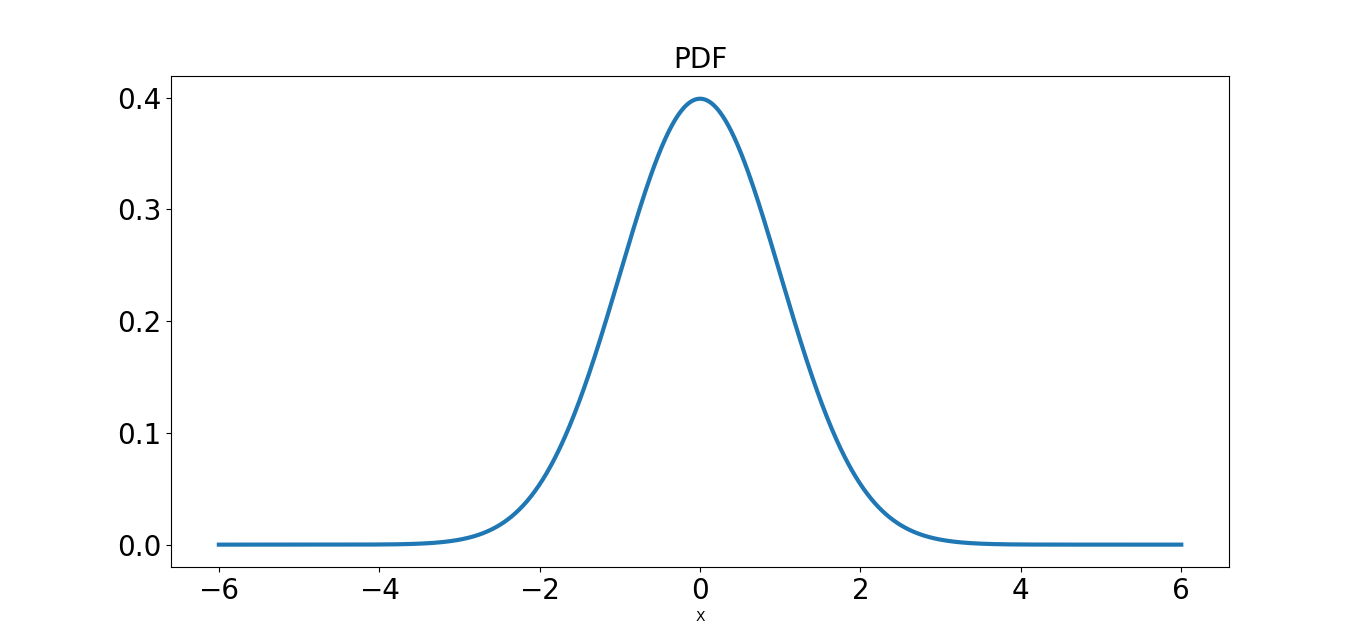
\includegraphics[width=80mm]{pdf_quiz6.png}
\end{subfigure}
\begin{subfigure}{0.49\textwidth}
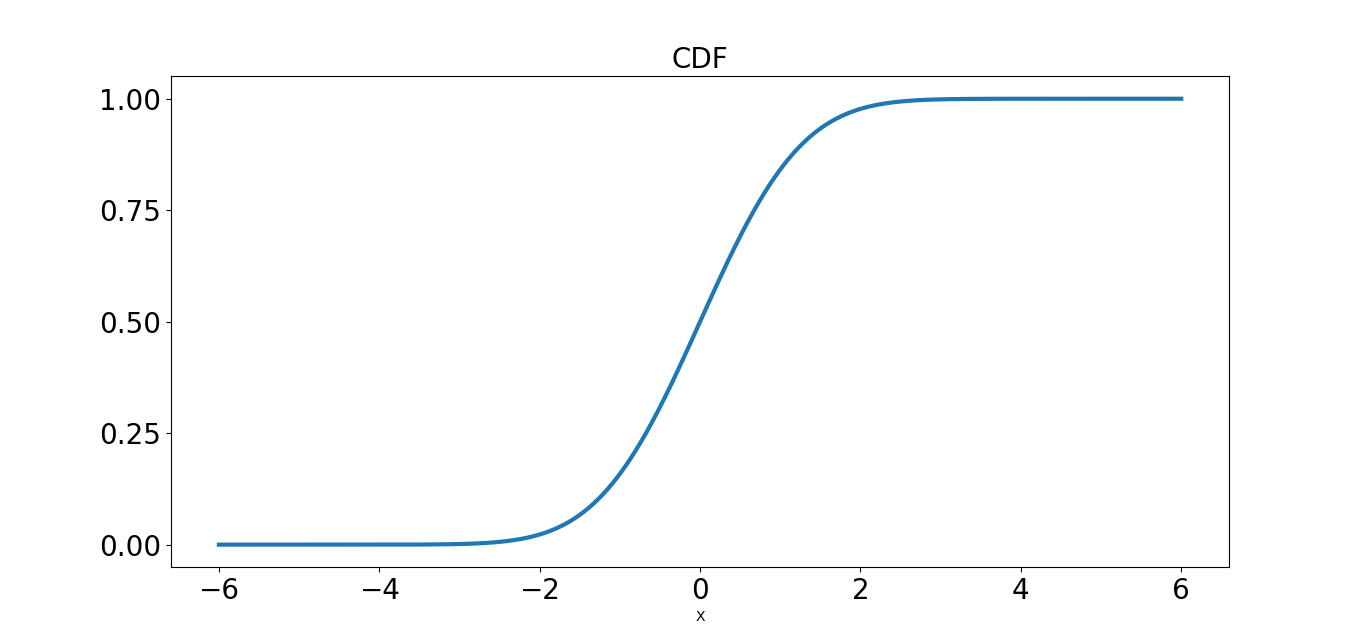
\includegraphics[width=80mm]{cdf_quiz6.png}
\end{subfigure}
\end{figure}

اگر چگالی احتمال و توزیع تجمعی متغیر $Y=2-X$ را بر حسب چگالی احتمال و توزیع تجمعی متغیر $X$ بیابید و آنها را رسم کنید.

\Q
از دو جامعه ی آماری بزرگ، یک آزمون علمی 100 نمره ای گرفته شده است. مشاهده شده که نمرات افراد این دو جامعه، به ترتیب از دو توزیع گوسی با میانگین های 59 و 73 و واریانس های 9 و 16 پیروی می کند.

الف) کدام یک از این دو جامعه به طور متوسط دارای سطح علمی بالاتری است؟ چرا؟

ب) افراد کدام جامعه دارای سطح علمی نزدیک تری به یکدیگر هستند؟ (یا به عبارت دیگر، هم سطح ترند؟) چرا؟

\Q
الف) آیا چگالی احتمال یک متغیر تصادفی می تواند تابعی فرد باشد؟ توضیح دهید.

ب) گشتاور مرتبه $n$-ام یک متغیر تصادفی یکنواخت در بازه‌ی $[a,b]$ را به دست آورید.

\Q
الف) برای هر متغیر تصادفی $X$ و $s>0$ تحقیق کنید 
$$
\Pr\{X\ge a\}=\Pr\{e^{sX}\ge e^{sa}\}
$$
ب) به کمک نامساوی مارکوف ثابت کنید:
$$
\Pr\{X\ge x\}\le e^{-sx}\Phi_X(s)
$$

\Q
تعیین کنید به ازای چه مقادیری از $k$، هر یک از توابع زیر می تواند تابع توزیع تجمعی یک متغیر تصادفی باشد.

الف) 
$
F(x)=\begin{cases}
1-e^{-kx^2}&,\quad x\ge 0\\
0&,\quad x<0
\end{cases}
$
\quad,\quad
ب)
$
F(x)={e^x\over e^x+k}
$

پ)
$
F(x)=\begin{cases}
kx&,\quad 0\le x\le 1\\
1&,\quad x>1\\
0&,\quad x<0
\end{cases}
$
\quad,\quad
ت)
$
F(x)=\cos {\pi\over e^x+k}
$

ث)
$
F(x)=\begin{cases}
k-e^{x-x^2}&,\quad x\ge 0\\
0&,\quad x<0
\end{cases}
$

\Q
اگر $F(x)$ تابع توزیع تجمعی یک متغیر تصادفی پیوسته باشد، کدام یک از توابع زیر می‌توانند تابع توزیع تجمعی یک متغیر تصادفی باشند؟ سپس برای هر تابع توزیع تجمعی، مقدار 
$\Pr\{1<X\le 2\}$
را بیابید (راهنمایی: از خواص تابع توزیع تجمعی بهره بگیرید.).

الف) 
$
F(x^2)
$
\quad,\quad
ب) 
$
F(x^3)
$
\quad,\quad
پ) 
$
1-F(-x)
$
\quad,\quad
ت) 
$
F^n(x)
$
برای هر مقدار طبیعی از $n$
\quad,\quad
ث) 
$
\sin\left[{\pi\over 2}F(x)\right]
$

\Q
تعیین کنید به ازای چه مقادیری از $k$، هر یک از توابع زیر می تواند چگالی احتمال یک متغیر تصادفی باشد. سپس برای هر چگالی احتمال، مقادیر 
$\Pr\{X=1\}$
و
$\Pr\left\{X<{1\over 2}\right\}$
را بیابید.

الف) 
$
f(x)=\begin{cases}
1/x^k&,\quad x\ge 1\\
0&,\quad x<0
\end{cases}
$
\quad,\quad
ب)
$
f(x)=\begin{cases}
kxe^{-x}&,\quad x\ge 0\\
0&,\quad x<0
\end{cases}
$

پ)
$
f(x)=\begin{cases}
\sin x&,0\le x\le k\\
0&,\quad \text{سایر جاها}
\end{cases}
$
\quad,\quad
ت)
$
f(x)=k\delta(x-1)+(1-k)\delta(x)
$

ث)
$
f(x)=\begin{cases}
k\delta(x-1)&,\quad x=1\\
x&,\quad 0<x<1\\
0&,\quad \text{سایر جاها}
\end{cases}
$
(به عبارت دیگر، تابع در نقطه‌ی $x=1$ دارای ضربه‌ای به مساحت $k$ است)



\Q
یک سامانه دارای 70 قطعه است. پیشامد اینکه هر قطعه پس از شروع به کار در زمان 0، در بازه‌ی 
$
(0,x)
$
دچار خرابی گردد، یک متغیر تصادفی با چگالی احتمال زیر است:
$$
f(x)=\begin{cases}
{1\over T}e^{-{x\over T}}&,\quad x\ge 0\\
0&,\quad x<0
\end{cases}
$$
احتمال آن را بیابید که بیش از 65 قطعه از این سیستم در بازه‌ی 
$
\left(0,{T\over 4}\right)
$
 دچار خرابی نشوند.

\Q
اگر 
$x_u$،
صدک-$u$ متغیر تصادفی 
$X$
باشد، در این صورت مقدار 
$x_u$
را به ازای 
$u=0.2,0.4,0.6,0.8$
برای توابع چگالی احتمال زیر به دست آورید.

الف)
$
f(x)=\begin{cases}
1&,\quad 0\le x\le 1\\
0&,\quad \text{سایر جاها}
\end{cases}
$
\quad,\quad
ب)
$
f(x)=\begin{cases}
2e^{-2x}&,\quad x\ge 0\\
0&,\quad \text{سایر جاها}
\end{cases}
$

\Q
زمان خرابی یک لامپ، یک متغیر تصادفی با چگالی احتمال زیر است،
$$
f_X(x)={1\over\lambda}e^{-{x\over\lambda}}\quad,\quad x>0
$$

الف) احتمال آن که این لامپ، به مدت حداکثر
$
2\lambda
$
عمر کند، چقدر است؟

ب) احتمال آن که این لامپ بیش از 
$
3\lambda
$
و کمتر از 
$
3.5\lambda
$
عمر کند چقدر است؟

\Q
یک متغیر تصادفی دارای چگالی احتمال زیر است،
$$
f_X(x)=\begin{cases}
6x^2(1-x)&,\quad 0\le x\le1\\
k\delta(x+1)&,\quad x=-1\\
0&,\quad \text{سایر جاها}
\end{cases}
$$
به عبارت دیگر، چگالی احتمال دارای ضربه ای به اندازه $k$ در $x=-1$ است.

الف) مقدار $k$ را بیابید.

ب) تابع توزیع تجمعی را به دست آورید و آن را رسم کنید.

پ) مقدار احتمال های 
$\Pr\{-2< X\le {1\over2}\}$
و
$\Pr\{0< X\le {1\over2}\}$
چقدر است؟

\Q
فرض کنید متغیر تصادفی $X$ دارای توزیع یکنواخت بین 0 و 1 است. در این صورت، تابع توزیع تجمعی و چگالی احتمال هر یک از متغیرهای تصادفی زیر را بیابید. سپس، مقادیر احتمال های 
$\Pr\{X\le {2\over 3}\}$
و
$\Pr\{Y\le {1\over \sqrt3}\}$
را از روی چگالی‌های احتمال $X$ و $Y$ بیابید و با هم مقایسه کنید. نتیجه مقایسه را توضیح دهید.


الف)
$
Y=X^2
$
\quad,\quad
ب)
$
Y=-\ln (1-X)
$
\quad,\quad
پ)
$
Y=\tan\pi (X-{1\over 2})
$

\Q
اگر تابع توزیع تجمعی متغیر تصادفی $X$ را با $F(x)$ نشان دهیم، توابع توزیع تجمعی متغیرهای تصادفی زیر را برحسب $F(x)$ دست آورید.

الف)
$Y=|X|$
\quad,\quad
ب)
$
Y=\begin{cases}
0&,\quad X\le0\\
1&,\quad X>0
\end{cases}
$
\quad,\quad
پ)
$Y=X^2-2X$

\Q
تابع جرم احتمال متغیر تصادفی $X$ دارای خاصیت زیر است:
$$6\Pr\{X=k+2\}-5\Pr\{X=k+1\}+\Pr\{X=k\}=0\quad,\quad k=1,2,\cdots$$
همچنین 
$\Pr\{X=1\}=\frac{7}{12}$.
در این صورت، چگالی جرم احتمال متغیر $X$ را بیابید.

\Q
متغیر تصادفی $X$ دارای چگالی احتمال زیر است:
$$f(x)=\frac{a}{2}e^{-ax}+\frac{1}{2}e^{-x}\quad,\quad x>0.$$
مقدار $a$ را به گونه ای بیابید به طوری که
$\mathbb{E}\{X\}=5$.

\Q
برای هر یک از توابع زیر، محدوده مقادیر $k$ را به گونه ای تعیین کنید که تابع مورد نظر، یک تابع توزیع انباشته باشد. سپس، چگالی احتمال را بیابید.

الف)
$F(x)=\frac{1}{e^{-kx}+1}$
\quad,\quad
ب)
$
F(x)=\begin{cases}
0&,\quad x<0\\
1-e^{-x-k\sin x}&,\quad x\ge0
\end{cases}
$

پ)
$
F(x)=\begin{cases}
0&,\quad x<0\\
1+xe^{-kx}&,\quad x\ge 0
\end{cases}
$

ت)
$
F(x)=\begin{cases}
0&,\quad x<0\\
\frac{1}{2}&,\quad 0\le x<1\\
1-\frac{1}{2}e^{k-kx}&,\quad x\ge 1
\end{cases}
$

\Q
برای بخش های الف و ت سوال پیش، مقادیر میانه، صدکهای 25ام و 75ام و همچنین احتمال‌های
$\Pr\{X=0\}$
و
$\Pr\{0< X\le 2\}$
را بیابید.

\Q
یک تاس را پرتاب می‌کنیم. اگر زوج آمد، عدد آن را یادداشت می‌کنیم و اگر فرد آمد، عددی را به تصادف از بازه‌ی 
$[1,6]$
انتخاب کرده و آن را یادداشت می‌کنیم. اگر متغیر تصادفی 
$X$،
نشان دهنده‌ی عدد یادداشت شده باشد، چگالی احتمال و تابع توزیع انباشته‌ی آن را به دست آورده و رسم کنید. سپس، مقدار 
$\Pr\{1\le X\le 3\}$
را بیابید.



\Q
فرض کنید متغیر تصادفی $X$، از توزیع نمایی با پارامتر $\lambda=1$ پیروی کند. در این صورت، چگالی احتمال متغیر تصادفی $Y$ را در حالت های زیر بیابید.

الف)
$
Y=e^X
$
\quad,\quad
ب)
$
Y=X^\alpha
$
که
$
\alpha
$
عدد ثابت مثبتی است.

پ)
$
Y=\lfloor X\rfloor
$

\Q
فرض کنید $X$، یک متغیر تصادفی باشد که از توزیع زیر پیروی می‌کند:
$$
f_X(x)=\begin{cases}
kx&,\quad 0<x<1\\
\frac{1}{2}\delta(x)&,\quad x=1\\
0&,\quad \text{جاهای دیگر}
\end{cases}
$$

الف) مقدار مناسب $k$ را بیابید.
\quad,\quad
ب) مقدار 
$
\mathbb{E}\{X\}
$
را محاسبه کنید.

پ) مقدار 
$
\mathbb{E}\{e^{aX}\}
$
را به دست آورید که $a$ عدد حقیقی دلخواهی است.

\Q
متغیر تصادفی $X$ از توزیع زیر پیروی می‌کند:
$$
f_X(x)=\begin{cases}
2xe^{-x^2}&,\quad x>0\\
0&,\quad \text{جاهای دیگر}\\
\end{cases}
$$
متغیر تصادفی
$
Y=X^2
$
مفروض است.

الف) چگالی احتمال $Y$ را به دست آورید.
\quad,\quad
ب) امید ریاضی $X$ را بیابید.

پ) امید ریاضی $Y$ را از روی چگالی احتمال آن و مقدار 
$
\mathbb{E}\{X^2\}
$
را از قضیه‌ی اساسی امید ریاضی محاسبه کرده و با هم مقایسه کنید.

ت) مقادیر
$
\Pr\{X<\frac{1}{2}\}
$
و
$
\Pr\{Y<\frac{1}{4}\}
$
را به ترتیب از روی چگالی های احتمال 
$
X
$
و
$
Y
$
به دست آورده و با هم مقایسه کنید.

\Q
برای هر یک از توزیع های زیر، مقدار 
$
\Pr\{X\ge \alpha\}
$
را به دست آورده و همچنین، یک کران بالا برای این احتمال برای هر توزیع با کمک نامساوی مارکوف به دست آورید. سپس مقدار دقیق احتمال و کران آن را مقایسه کنید.

الف)
$
f(x)=e^{-x}\quad,\quad x>0
$
\quad,\quad
ب)
$
f(x)=\frac{1}{\ln 2}\frac{1}{1+e^x}\quad,\quad x>0
$

پ)
$
f(x)=xe^{-x}\quad,\quad x>0
$

\Q
برای توزیع‌های بخش های الف و پ سوال پیش، مقدار واریانس را به دست آورید.

\Q
برای هر یک از توزیع های زیر، تابع مولد گشتاور را یافته و سپس از روی آن، مقدار 
$
\mathbb{E}\{X^2\}
$
را بیابید.

الف)
$
f(x)=\begin{cases}
1-x&,\quad 0<x<1\\
\frac{1}{2}\delta(x-1)&,\quad x=1
\end{cases}
$

ب)
$
f(x)=\begin{cases}
\cos x&,\quad 0<x<\frac{\pi}{2}\\
0&,\quad \text{جاهای دیگر}
\end{cases}
$

پ)
$
\Pr\{X=x\}=
\begin{cases}
\frac{n}{2^{n+1}}&,\quad n\in\Bbb N\\
0&,\quad \text{جاهای دیگر}
\end{cases}
$

ت)
$
X
$
متغیر تصادفی حاصل ضرب دو عدد رو آمده در پرتاب دو تاس به طور مستقل است.

\Q
برای هر یک از متغیرهای تصادفی زیر، واریانس را به دست آورید.

الف) 
$
f_X(x)=\begin{cases}
e^{-x}&,\quad x>1\\
0&,\quad x\le1
\end{cases}
$

ب) 
$
f_X(x)=\begin{cases}
\sin x&,\quad 0<x<{\pi\over 2}\\
0&,\quad \text{سایر جاها}
\end{cases}
$

پ)
$
f_X(x)=
\begin{cases}
{2\over x^3}&,\quad x>1\\
0&,\quad \text{سایر جاها}
\end{cases}
$

ت) X یک متغیر تصادفی گسسته است و 
$
\Pr\{X=i\}=2({1\over 3})^i
$
برای 
$
i\in\Bbb N
$

\Q
برای قسمت های الف و ت سوال 1، ابتدا تابع مولد گشتاور را محاسبه نموده و سپس از روی آن، میانگین و واریانس را به دست آورید.

\Q
برای قسمت های الف و ب سوال 1، میانگین متغیر تصادفی $e^{-X}$ را بیابید.

\Q
برای متغیر تصادفی $X$ با چگالی‌های احتمال زیر، ابتدا تابع مولد گشتاور را یافته و سپس از روی آن، مقادیر میانگین، واریانس و 
$\text{var}\left\{X|X>\frac{1}{2}\right\}$
 را بیابید.

الف)
$
f_X(x)=\begin{cases}
{1\over 2}\sin x&,\quad 0<x<\pi\\
0&,\quad \text{سایر جاها}
\end{cases}
$

ب)
$
f_X(x)=\begin{cases}
\cos x&,\quad 0<x<{\pi\over 2}\\
0&,\quad \text{سایر جاها}
\end{cases}
$

پ)
$
f_X(x)=\begin{cases}
xe^{-x}&,\quad x>0\\
0&,\quad \text{سایر جاها}
\end{cases}
$

ت)
$
f_X(x)=\begin{cases}
\frac{3}{7}x^2&,\quad 1<x<2\\
0&,\quad \text{سایر جاها}
\end{cases}
$

ث)
$
f_X(x)=\begin{cases}
\frac{1}{2}\delta(x-1)&,\quad x=1\\
x&,\quad 0<x<1\\
0&,\quad \text{سایر جاها}
\end{cases}
$



%%%%%%%%%%%%%%%%%%%%%%%%%%%%%%%%%%%%%%
%%%%%%%%%%%%%%%%%%%%%%%%%%%%%%%%%%%%%%
%%%%%%%%%%%%%%%%%%%%%%%%%%%%%%%%%%%%%%
%%%%%%%%%%%%%%%%%%%%%%%%%%%%%%%%%%%%%%
%%%%%%%%%%%%%%%%%%%%%%%%%%%%%%%%%%%%%%

\chapter{متغیرهای تصادفی توأم}

\Q
فرض کنید $X$ و $Y$ دو متغیر تصادفی مستقل برنولی به ترتیب با پارامترهای $1\over 2$ و $p$ باشند. ثابت کنید
$Z=X\oplus Y \mod 2$
و
$Z=XY$
 دارای توزیع برنولی با پارامتر ${1\over 2}p$ هستند.

%%%%%%%%%%%%%%%%%%%%%%%%%%%%%%%%%%%%%%

\Q
اگر $X$ و $Y$ دو توزیع چندجمله ای به ترتیب با پارامترهای 
$
(n_1,p)
$
 و 
$
(n_2,p)
$
 باشند، ثابت کنید توزیع $X+Y$ دوجمله ای با پارامترهای $(n_1+n_2,p)$ است.

%%%%%%%%%%%%%%%%%%%%%%%%%%%%%%%%%%%%%%

\Q
تابع چگالی احتمال توام دو متغیر تصادفی $X$ و $Y$ به صورت زیر است:
$$
f(x,y)=
\begin{cases}
k(4-x-y) &,\quad 1 < x < 2\ \ ,\ \   0 < y < 2 \\
0 &,\quad \text{\rl{در غیر این صورت}}
\end{cases}
$$
الف) مقدار مناسب $k$ را بیابید.

ب) با مقدار $k$ به دست آمده در قسمت قبل، مقدار 
$
\EX \{XY\}
$
 را به دست آورید.

%%%%%%%%%%%%%%%%%%%%%%%%%%%%%%%%%%%%%%

\Q
تابع چگالی احتمال توام دو متغیر تصادفی $X$ و $Y$ به صورت زیر است:
$$
f(x,y)=
\begin{cases}
1 &,\quad |x|+2|y|<1\\
0 &,\quad |x|+2|y|\ge 1
\end{cases}
$$
الف)  چگالی های احتمال حاشیه ای $X$ و $Y$ را به دست آورید. همچنین ناهمبستگی، استقلال و تعامد این دو متغیر تصادفی را تحقیق کنید.

ب) چگالی احتمال $X+Y$ را به دست آورید.

%%%%%%%%%%%%%%%%%%%%%%%%%%%%%%%%%%%%%%

\Q
یک قطار و اتوبوس به طور تصادفی و مستقل از هم بین ساعات 5 تا 6 وارد یک ایستگاه می‌شوند. فردی نیز به طور تصادفی بین ساعت 5 تا $5:30$ وارد همان ایستگاه می‌شود.

الف) احتمال آن که فرد بیش از 10 دقیقه منتظر قطار و اتوبوس شود چقدر است؟

ب) اگر قطار و اتوبوس هر یک 10 دقیقه در ایستگاه تاخیر داشته باشند، احتمال با هم بودن آنها در ایستگاه چفدر است؟

پ) اگر فرد پس از ساعت $5:15$ به ایستگاه برسد، با چه احتمالی به هیچ یک نمی‌رسد؟

%%%%%%%%%%%%%%%%%%%%%%%%%%%%%%%%%%%%%%

\Q
یک قطار و اتوبوس به طور تصادفی و مستقل از هم بین ساعات 6 تا 7 صبح وارد ایستگاهی می شوند. فردي نیز به طور تصادفی بین ساعات 5:50 تا 6:50 وارد همان ایستگاه می شود.

الف) احتمال اینکه فرد بیش از 10 دقیقه منتظر قطار ویا اتوبوس بماند چقدر است؟

ب) احتمال اینکه این فرد به هیچ یک از قطار یا اتوبوس نرسد چقدر است؟

%%%%%%%%%%%%%%%%%%%%%%%%%%%%%%%%%%%%%%

\Q
اگر $X$ و $Y$، دو متغیر تصادفی نرمال با میانگین 0 و واریانس 1 باشند به گونه ای که 
$
\text{\lr{cov}}(X,Y)=0.5
$
، در این صورت مقدار $a$  را به گونه ای بیابید که $X+aY$ و $X+2Y$ مستقل از هم باشند و در این صورت، واریانس هر یک را بیابید.

%%%%%%%%%%%%%%%%%%%%%%%%%%%%%%%%%%%%%%

\Q
تابع چگالی احتمال توام دو متغیر تصادفی $X$ و $Y$ به صورت زیر است:
$$
f(x,y)=
\begin{cases}
k(4-x-y) &,\quad 1 < x < 2\ \ ,\ \   0 < y < 2 \\
0 &,\quad \text{\rl{در غیر این صورت}}
\end{cases}
$$
الف) مقدار مناسب $k$ را بیابید.

ب) با مقدار $k$ به دست آمده در قسمت قبل، مقدار 
$
\EX \{XY\}
$
 را به دست آورید.

%%%%%%%%%%%%%%%%%%%%%%%%%%%%%%%%%%%%%%

\Q
تابع چگالی احتمال توأم دو متغیر تصادفی $X$ و $Y$ به صورت زیر است:
$$
f_{X,Y}(x,y)=\begin{cases}
k&,\quad x-1<y<x\ \ ,\ \ 0<x<2\ \ ,\ \ 0<y<1
\\0&,\quad \text{در غیر این صورت}
\end{cases}
$$
که $k$ ثابت است.

الف) مقدار $k$ را به دست آورید.

ب) نشان دهید $Y$ و $X-Y$ از هم مستقل هستند.

%%%%%%%%%%%%%%%%%%%%%%%%%%%%%%%%%%%%%%

\Q
یک قطار و یک اتوبوس بین ساعت 9 و 10 در زمانی تصادفی وارد ایستگاه می‌شوند. قطار 10 دقیقه و اتوبوس $x$ دقیقه توقف دارند. $x$ را طوری تعیین کنید که احتمال با هم بودن قطار و اتوبوس برابر $0.5$ باشد.

%%%%%%%%%%%%%%%%%%%%%%%%%%%%%%%%%%%%%%

\Q
دایره‌ی واحد را با مرکز مبدا مختصات در نظر بگیرید.

الف) نقطه ای به تصادف از داخل این دایره انتخاب می شود. اعداد 
$
0<r_0<1
$
 و 
$
0<\phi_0<2\pi
$ 
را در نظر بگیرید.  اگر مختصات قطبی این نقطه را با 
$
(r,\phi)
$
 نشان دهیم، با چه احتمالی داریم 
$
r_0<r<r+\Delta r_0
$
 و 
$
\phi_0<\phi<\phi_0+\Delta\phi_0
$
؟

ب) ابتدا قطری از دایره را به تصادف انتخاب کرده و سپس نقطه ای از این قطر را به تصادف بر می‌گزینیم. اگر مختصات قطبی این نقطه را با 
$
(r,\phi)
$
 نشان دهیم، با چه احتمالی داریم 
$
r_0<r<r+\Delta r_0
$
 و 
$
\phi_0<\phi<\phi_0+\Delta\phi_0
$
؟

پ) تابع چگالی احتمال نقطه را در هر دو حالت قسمت های الف و ب به دست آورید.

%%%%%%%%%%%%%%%%%%%%%%%%%%%%%%%%%%%%%%

\Q
(ناوردایی متغیرهای تصادفی گوسی تحت عمل جمع)

الف) فرض کنید $X$ و $Y$ دو متغیر تصادفی با توابع چگالی احتمال زیر باشند:
\[
f_X(x)={1\over \sqrt{2\pi\sigma_X^2}}\exp\left(-{x^2\over 2\sigma_X^2}\right)
\]
\[
f_Y(y)={1\over \sqrt{2\pi\sigma_Y^2}}\exp\left(-{y^2\over 2\sigma_Y^2}\right)
\]
ثابت کنید متغیر تصادفی $X+Y$ از توزیع زیر پیروی می کند:
\[
f_{X+Y}(u)={1\over \sqrt{2\pi[\sigma_X^2+\sigma_Y^2]}}\exp\left(-{u^2\over 2\pi[\sigma_X^2+\sigma_Y^2]}\right)
\]
ب) رابطه‌ی کلی تری را که می‌توان از تعمیم قسمت الف استنتاج کرد، بنویسید.

%%%%%%%%%%%%%%%%%%%%%%%%%%%%%%%%%%%%%%

\Q
برای هر کدام از توابع زیر که می‌توانند چگالی احتمال مشترک دو متغیر تصادفی باشند، ثابت مناسب $k$ و مقادیر
$\Pr\{X>0\}$
و
$\Pr\{X+Y>0\}$
 را بیابید. همچنین برای قسمت های ث) و ج)، چگالی احتمال متغیر تصادفی $X$ را به دست آورید.

الف) 
$
f(x,y)={k\over 1+x^2+y^2}
$

ب)
$
f(x,y)=e^{a(x^2+y^2)}
$

پ)
$
f(x,y)=\begin{cases}
k&,\quad x^2+y^2<1
\\
0&,\quad \text{\rl{در غیر این صورت}}
\end{cases}
$

ت)
$
f(x,y)=\begin{cases}
k-k\sqrt{x^2+y^2}&,\quad x^2+y^2<1
\\
0&,\quad \text{\rl{در غیر این صورت}}
\end{cases}
$

ث)
$
f(x,y)=\begin{cases}
xy&,\quad 0<x<k\quad,\quad 0<y<k
\\
0&,\quad \text{\rl{در غیر این صورت}}
\end{cases}
$

ج)
$
f(x,y)=\begin{cases}
1&,\quad x>0\ \ ,\ \ y>0\ \ ,\ \ x+y<a
\\
0&,\quad \text{\rl{در غیر این صورت}}
\end{cases}
$

(راهنمایی: ابتدا تحقیق کنید اگر $f(x,y)$ تابعی از $x^2+y^2$ باشد، داریم 
$$\Pr\{aX+bY>0\}=\Pr\{X>0\}\quad,\quad a^2+b^2\ne 0$$)

%%%%%%%%%%%%%%%%%%%%%%%%%%%%%%%%%%%%%%

\Q
دو متغیر تصادفی $X$ و $Y$ با چگالی احتمال توأم زیر مفروضند. در این صورت، مقدار $\alpha$ را به گونه ای بیابید که این دو متغیر تصادفی ناهمبسته شوند.
$$
f_{XY}(x,y)=\begin{cases}
\frac{x^2}{2}+y^2+\alpha xy&,\quad -1<x<1\ \ ,\ \ -1<y<1\\
0&,\quad \text{سایر جاها}
\end{cases}
$$

%%%%%%%%%%%%%%%%%%%%%%%%%%%%%%%%%%%%%%

\Q
دو متغیر تصادفی $X$ و $Y$ با چگالی احتمال توأم زیر مفروضند. در این صورت، تابع توزیع تجمعی توأم این دو متغیر تصادفی را بیابید.
$$
f_{XY}(x,y)=\begin{cases}
ye^{1-xy}&,\quad x>1\ \ ,\ \ y>1\\
0&,\quad \text{سایر جاها}
\end{cases}
$$

%%%%%%%%%%%%%%%%%%%%%%%%%%%%%%%%%%%%%%

\Q
دو نفر به طور مستقل از هم و کاملا تصادفی بین ساعت 4 و 5 وارد فروشگاهی می شوند و هر یک پس از 10 دقیقه، از آن خارج می شوند. احتمال آن که این دو نفر یکدیگر را در فروشگاه ملاقات کنند چقدر است؟

%%%%%%%%%%%%%%%%%%%%%%%%%%%%%%%%%%%%%%

\Q
جدول زیر را برای متغیرهای تصادفی $X$ و $Y$ در نظر بگیرید:
\begin{table}[h]
\centering
\Large
\lr{
\begin{tabular}{|c|c|c|}
\hline
\backslashbox{$X$}{$Y$}&0&1\\\hline
0&$\frac{1}{2}-\theta$&$\theta$\\\hline
1&$\theta$&$\frac{1}{2}-\theta$\\\hline
\end{tabular}
}
\end{table}

الف) توابع توزیع احتمال حاشیه‌ای متغیرهای $X$ و $Y$ را به دست آورید.

ب) به ازای چه مقدار $\theta$ داریم
$
P(X=Y)=1
$
؟

پ) به ازای چه مقدار $\theta$ داریم
$
P(X=x,Y=y)=P(X=x)P(Y=y)
$
؟

%%%%%%%%%%%%%%%%%%%%%%%%%%%%%%%%%%%%%%

\Q
در پرتاب دو تاس سالم و متمایز، متغیر تصادفی $X$ را مجموع اعداد رو آمده و $Y$ را تعداد 6 های رو آمده در نظر بگیرید.

الف) مقادیر 
$
\Pr\{X=1,Y=7\}
$
و
$
\mathbb{E}\{XY\}
$
 چقدر است؟

ب) آیا این دو متغیر تصادفی ناهمبسته اند؟

%%%%%%%%%%%%%%%%%%%%%%%%%%%%%%%%%%%%%%

\Q
در جدول زیر که توزیع احتمال را برای متغیر های تصادفی $X$ و $Y$ نشان می‌دهد،
\begin{table}[h]
\centering
\Large
\lr{
\begin{tabular}{|c|c|c|}
\hline
\backslashbox{$X$}{$Y$}&0&1\\\hline
0&$p_1$&$p_2$\\\hline
1&$p_3$&$p_4$\\\hline
\end{tabular}
}
\end{table}

الف) مقدار 
$
\text{\lr{cov}}(X,Y)
$
 را به دست آورید و تحقیق کنید چه زمانی این کمیت صفر است.

ب) آیا برای این دو متغیر تصادفی، ناهمبستگی، استقلال را نتیجه می دهد؟ اگر چنین است، نشان دهید و اگر چنین نیست، مثالی برای مقادیر 
$
p_1,p_2,p_3,p_4
$
 بزنید که ناهمبستگی، استقلال را نتیجه نمی‌دهد (دقت داشته باشید که جمع احتمالات برابر یک است و احتمالات نامنفی اند).

%%%%%%%%%%%%%%%%%%%%%%%%%%%%%%%%%%%%%%

\Q
چگالی احتمال زیر را در نظر بگیرید:
$$
f_{X,Y}(x,y)=\begin{cases}
1+\alpha\sin[2\pi(x+y)]&,\quad 0\le x\le1,0\le y\le1
\\0&,\quad \text{در غیر این صورت}
\end{cases}
$$
که $\alpha$ مقدار مناسبی است.

الف) کوواریانس این دو متغیر تصادفی را به دست آورید. آیا این دو متغیر تصادفی ناهمبسته هستند؟

ب) مقادیری از $\alpha$ را بیابید که این دو متغیر تصادفی مستقل باشند.

%%%%%%%%%%%%%%%%%%%%%%%%%%%%%%%%%%%%%%

\Q
تابع چگالی احتمال توام زیر را در نظر بگیرید:
$$
f_{X,Y}(x,y)={1\over 2\pi \sqrt{1-\rho^2}}\exp\left[-{1\over 2}\cdot{1\over 1-\rho^2}(x^2+y^2-2\rho xy)\right]
$$
الف) ثابت کنید $X$ (و مشابها همچنین $Y$) دارای توزیع نرمال با میانگین صفر و واریانس $1$ است.

ب) ثابت کنید اگر $\rho=0$، در این صورت متغیرهای تصادفی $X$ و $Y$ مستقل هستند.

پ) ثابت کنید اگر متغیرهای تصادفی $X$ و $Y$ مستقل باشند آنگاه $\rho=0$.

ت) تابع چگالی احتمالی که در صورت این سوال تعریف شد، حالت خاصی از چگالی احتمال چند متغیره‌ی نرمال است.

ضریب همبستگی $\rho$ در حالت دو متغیره، میزان همبستگی دو متغیر تصادفی را نشان می دهد. ابتدا تحقیق کنید به ازای چه مقداری از $\rho$، این چگالی احتمال، دایروی-متقارن خواهد بود. چگالی احتمال دو متغیره را به ازای مقادیر 
$\rho=-0.5,\rho=0,\rho=0.5$
 ترسیم کنید. به طور شهودی چگونه می توان از روی نمودارها، به میزان همبستگی این دو متغیر تصادفی پی برد؟

این تابع چگالی را به صورت دیگری نیز می توان نوشت:
$$
f(x,y)={1\over \sqrt{(2\pi)^2}\det(\Sigma)}\exp\left[-{1\over 2}\cdot([x,y]\Sigma^{-1}[x,y]^T)\right]
$$
که بردار $[x,y]$ یک بردار سطری دوتایی است و 
$
\Sigma=\begin{bmatrix}
1&\rho\\
\rho&1
\end{bmatrix}
$.
ماتریس $\Sigma$ در متغیرهای تصادفی نرمال توأم، مفهوم مهمی است و ماتریس کوواریانس نام دارد.

به ازای هر یک از مقادیر 
$\rho=-0.5,\rho=0,\rho=0.5$
 و به کمک دستور 
\lr{mvnrnd()}
 در متلب، 1000 جفت داده‌ی تصادفی تولید و آنها را در یک نمودار پراکندگی ترسیم کنید (پس از اجرای دستور فوق در متلب به شیوه ی مناسب، 1000 داده‌ی تصادفی برای $X$ و 1000 داده‌ی تصادفی برای $Y$ خواهید داشت. کافی است $Y$ را برحسب $X$ رسم کنید تا به نمودار پراکندگی برسید. همچنین می توانید از \lr{Help} متلب برای توضیحات بیشتر در مورد \lr{mvnrnd()} بهره ببرید). چگونه از روی نمودار پراکندگی می توان میزان همبستگی دو متغیر تصادفی را نشان داد؟ چه شهودی در آن نهفته است؟ (بسیار مهم است که در این تحقیق، تحلیل و دیدگاه خود را نیز ذکر بفرمایید.)

هنگامی که $\rho=1$، توضیح دهید چه اتفاقی می افتد؟ تفاوت آن با حالت $\rho=-1$ چیست؟ آیا همچنان می‌توان از چگالی احتمال داده شده استفاده کرد؟ چرا؟

%%%%%%%%%%%%%%%%%%%%%%%%%%%%%%%%%%%%%%

\Q
برای هر یک از چگالی احتمال های توام داده شده‌ی زیر، موارد 
$
f_X(x)
$
،
$
\mathbb{E}\{X\}
$
و
$
\mathbb{E}\{XY\}
$
را به دست آورید.

الف) 
$
f_{X,Y}(x,y)=\frac{1}{\pi}e^{-x^2-y^2}
$

ب) 
$
f_{X,Y}(x,y)=\begin{cases}
\frac{3}{2}(1-|x-1|-|y-1|)&,\quad |x-1|+|y-1|<1\\
0&,\quad \text{سایر جاها}
\end{cases}
$

پ)
$
f_{X,Y}(x,y)=\begin{cases}
e^{1-x}&,\quad 0<x<y<1\\
0&,\quad \text{سایر جاها}
\end{cases}
$

ت) X و Y ، دو متغیر تصادفی گسسته (با مقادیر صحیح) اند و تابع جرم احتمال آنها به صورت زیر است،
$$
\Pr\{X=x,Y=y\}=\begin{cases}
\frac{1}{16}&,\quad x^2+y^2\le 10 \ \ ,\ \ x\ge y\\
0&,\quad \text{سایر جاها}
\end{cases}
.
$$

%%%%%%%%%%%%%%%%%%%%%%%%%%%%%%%%%%%%%%

\Q
ابتدا فرض کنید متغیرهای تصادفی $X$ و $Y$ دارای توزیع یکنواخت در بازه‌ی $[0,1]$ و مستقل هستند. توزیع احتمال متغیرهای تصادفی 

الف) $XY$
\quad,\quad
ب) $X+Y$
\quad,\quad
پ) $X\over Y$
\quad,\quad
ت) $\max\{X,Y\}$

ث) $\min\{X,Y\}$

را به دست آورید. سپس فرض کنید $X$ و $Y$ دو متغیر تصادفی نمایی و مستقل با پارامتر 1 باشند. توزیع احتمال هر یک از متغیرهای تصادفی قسمت ب و پ را بیابید.

\Q
تابع چگالی احتمال توام دو متغیر تصادفی $X$ و $Y$ به صورت زیر است:
$$
f_{XY}(x,y)=\begin{cases}
k&,\quad |x|+|y|<1\\
0&,\quad \text{\rl{در غیر این صورت}}
\end{cases}
$$
الف) مقدار مناسب $k$ را بیابید.
\quad,\quad
ب) کوواریانس و ضریب همبستگی $X$ و $Y$ را بیابید.

پ) ثابت کنید متغیرهای تصادفی $X+Y$ و $X-Y$ مستقل هستند و توزیع توام آنها را به دست آورید.
\quad,\quad
ت) توزیع $X$ و میانگین و واریانس آن را به دست آورید.

\Q
برای متغیر تصادفی $X$ که دارای توزیع زیر است
$$
f_X(x)=\begin{cases}
1&,\quad |x|<{1\over 2}\\
0&,\quad \text{\rl{در غیر این صورت}}
\end{cases}
$$
تابع مولد گشتاور را به دست آورده و از روی آن، $\mathbb{E}\{X^4\}$ را محاسبه نمایید.

\Q
توزیع مشترک دو متغیرتصادفی به صورت زیر است،
$$
f_{X,Y}(x,y)={1\over 2\pi \sqrt{1-\rho^2}}\exp\left[-{1\over 2}\cdot{1\over 1-\rho^2}(x^2+y^2-2\rho xy)\right]
$$
الف) ثابت کنید متغیر تصادفی $X+Y$ یک متغیر تصادفی نرمال است و سپس واریانس آن را به دست آورید. چه زمانی این واریانس بیشینه است و چرا؟ در شرایطی که واریانس بیشینه باشد، متغیرهای تصادفی $X$ و $Y$ چه رابطه‌ای دارند؟

ب) ثابت کنید به ازای $\rho=0$، متغیر تصادفی $\tan^{-1}{Y\over X}$ دارای توزیع یکنواخت در بازه‌ی 
$\left[-\frac{\pi}{2},\frac{\pi}{2}\right]$
خواهد بود.

\Q
برای هر یک از توابع دومتغیره‌ی زیر، محدوده مقادیر $k$ را به گونه ای بیابید که تابع مورد نظر، چگالی احتمال توأم دو متغیر تصادفی باشد و سپس، توزیع تجمعی توأم و مقدار $\Pr\left\{X+3Y<{1\over 3}\right\}$ را (در صورت وجود) بیابید. به ازای هر تابع توزیع تجمعی، آیا $X$ و $Y$ مستقلند؟

الف)
$
f(x,y)=
\begin{cases}
xy+kx+ky&,\quad 0<x<1,0<y<1\\
0&,\quad \text{سایر جاها}
\end{cases}
$

ب)
$
f(x,y)=
\begin{cases}
k\sin(x+3y)&,\quad 0<x<\frac{\pi}{2},0<y<\frac{\pi}{6}\\
0&,\quad \text{سایر جاها}
\end{cases}
$

پ)
$
f(x,y)=\begin{cases}
kxy(1-y)&,\quad 0<x<1,0<y<1\\
0&,\quad \text{سایر جاها}
\end{cases}
$

%پ) (امتیازی)
%
%$
%f(x,y)=
%\begin{cases}
%\frac{1}{2}&,\quad |x|^k+|y|^k<1\\
%0&,\quad \text{سایر جاها}
%\end{cases}
%$

\Q
برای هر یک از چگالی های احتمال زیر، مقادیر
$\Pr\{X\le 4,Y\le -2\}$
،
$\Pr\{X+Y\le 2\}$
و
$\Pr\{X=4Y\}$
را بیابید.

الف)
$
f_{XY}(x,y)=
\begin{cases}
\frac{1}{2}\sin (x+y)&,\quad 0<x<\frac{\pi}{2},0<y<\frac{\pi}{2}\\
0&,\quad \text{سایر جاها}
\end{cases}
$

ب)
$
f_{XY}(x,y)=
\begin{cases}
\frac{1}{2}\delta\left(\sqrt{(x+4)^2+(y+1)^2}\right)&,\quad x=-4,y=-1\\
\frac{1}{2}&,\quad 0<x<1,0<y<1\\
0&,\quad \text{سایر جاها}
\end{cases}
$

(دقت شود که همانگونه که 
$
\delta(x-x_0)
$
نشان دهنده‌ی ضربه ای در 
$
x=x_0
$
است، 
$
\delta(\sqrt{(x-x_0)^2+(y-y_0)^2})
$
نیز نشان دهنده‌ی ضربه ای در 
$
x=x_0,y=y_0
$
در دو بعد و دارای سطح زیر یک است.)

\Q
برای چگالی احتمال توأم زیر، مقادیر
$
\sigma_X^2
$،
$
\sigma_Y^2
$،
$
\Phi_X(s)
$،
$
\Phi_Y(s)
$
و چگالی احتمال متغیرهای تصادفی $XY$ و 
$
\max\{X,Y\}
$
 را محاسبه کنید.
$$
f_{X,Y}(x,y)=\begin{cases}
(xy-1)e^{1-xy}&,\quad x\ge 1,y\ge 1\\
0&,\quad \text{سایر جاها}
\end{cases}
$$

\Q
چگالی احتمال توأم زیر برای دو متغیر تصادفی $X$ و $Y$ داده شده است:
$$
f_{X,Y}(x,y)=\begin{cases}
\alpha+2(\frac{1}{\pi}-\alpha)(x^2+y^2)&,\quad x^2+y^2\le 1\\
0&,\quad \text{سایر جاها}
\end{cases}
$$

الف) محدوده‌ی مقادیر مجاز 
$
\alpha
$
را بیابید.

ب) به ازای چه مقدار از 
$
\alpha
$
، دو متغیر تصادفی 
$
X
$
و
$
Y
$
مستقل اند؟ ناهمبسته اند؟

پ) احتمال های
$
\Pr\{aX+bY\ge 0\}
$
و
$
\Pr\{XY\ge 0\}
$
را بیابید.

\Q
اگر چگالی احتمال مشترک دو متغیر تصادفی $X$ و $Y$ به صورت زیر باشد
\[
f(x,y)=\begin{cases}
12x^2&,\quad 0<x<y<1\\
0&,\quad \text{سایر جاها}
\end{cases}
\]
در این صورت مقدار 
$
\text{cov}(X,Y)
$
را بیابید.

\Q
سکه ای را 10 بار پرتاب می‌کنیم. متغیر تصادفی 
$X$،
تعداد دفعات رو آمدن سکه در 5 پرتاب اول و متغیر تصادفی $Y$، تعداد دفعات رو آمدن سکه در پرتاب های زوج است. احتمال 
$\Pr\{X=5Y\}$
را بیابید.

\Q
متغیر تصادفی $X$، دارای تابع جرم احتمال زیر است:
\rl{
\begin{table}[h]
\centering
\Large
\begin{tabular}{|c|c|c|c|c|}
\hline
$x$&$-1$&$0$&$1$&$2$\\\hline
$\Pr\{X=x\}$&$0.1$&$0.2$&$0.3$&$0.4$\\\hline
\end{tabular}
\end{table}
}

اگر داشته باشیم
$Y=X^2-1$،
در اینصورت مقدار
$\text{cov}(X,Y)$
را بیابید.

\Q
برای متغیرهای تصادفی $X$ و $Y$ با چگالی‌های احتمال توأم زیر،

$$
f_{X,Y}(x,y)=\begin{cases}
x+ky&,\quad 0<x<1\ \ ,\ \ 0<y<1\\
0&,\quad \text{سایر جاها}
\end{cases}
$$

$$
f_{X,Y}(x,y)=\begin{cases}
kx&,\quad 0<x<1\ \ ,\ \ 0<x<y<1\\
0&,\quad \text{سایر جاها}
\end{cases}
$$

$$
f_{X,Y}(x,y)=\begin{cases}
kx&,\quad 0<y<1\ \ ,\ \ 0<y<x<1\\
0&,\quad \text{سایر جاها}
\end{cases}
$$

$$
f_{X,Y}(x,y)=\begin{cases}
kx&,\quad x+y<1 \ \ ,\ \ x>0 \ \ , \ \ y>0\\
0&,\quad \text{سایر جاها}
\end{cases}
$$

$$
f_{X,Y}(x,y)=\begin{cases}
k(1+x+y)&,\quad 1<x<2\ \ , \ \ 0<y<1\\
0&,\quad \text{سایر جاها}
\end{cases}
$$

الف) مقدار مناسب $k$ را بیابید.

ب) توزیع حاشیه ای 
$
f_X(x)
$
را پیدا کنید.

پ) مقدار 
$
\text{cov}(X,Y)
$
را محاسبه کنید.

ت) استقلال دو متغیر تصادفی را بررسی کنید.

ث) چگالی احتمال $X+Y$ را بیابید.

\Q
سکه سالمی را 5 بار می اندازیم. تابع مولد گشتاور مشترک $X$ و $Y$ و مقدار
$\mathbb{E}\{X+Y|X=1\}$
را محاسبه کنید، اگر:

الف) $X$ تعداد رو آمدن ها در سه پرتاب اول و $Y$ تعداد پشت آمدن ها در سه پرتاب آخر باشد.

ب) $X$ تعداد روها در پرتاب های فرد و $Y$ تعداد پشت ها در سه پرتاب آخر باشد.

پ) $X$ تعداد پشت ها در پرتاب های زوج و $Y$ تعداد پشت ها در سه پرتاب آخر باشد.

ت) $X$ تعداد پشت ها و $Y$ تعداد رو ها در سه پرتاب آخر باشد.

ث) $X$ تعداد پشت ها و $Y$ تعداد رو ها در دو پرتاب اول باشد.

\Q
یک امتحان احتمال مهندسی به صورت آنلاین (و با رعایت پروتکل های بهداشتی!) به مدت 2 ساعت برگزار می‌شود. فرهاد و آرش، هر یک مستقل از دیگری و به تصادف در 10 دقیقه‌ی اول (با توزیع یکنواخت) وارد جلسه امتحان می‌شوند. اگر این دو نفر مستقل از هم در بازه‌ی 1 تا $1.5$ ساعت از شروع و با توزیع یکنواخت، امتحان خود را به پایان رسانده و از جلسه خارج شوند،

الف) با چه احتمالی فرهاد زودتر از آرش از جلسه امتحان خارج می شود؟

ب) اگر آرش زودتر از فرهاد به جلسه آمده باشد، با چه احتمالی حداکثر 15 دقیقه دیرتر از از جلسه خارج می‌شود؟

پ) با چه احتمالی آرش حداکثر 10 دقیقه پس از فرهاد از جلسه خارج می شود؟

ت) احتمال آن که فرهاد زودتر از آرش به جلسه آمده و زودتر از او خارج شود چقدر است؟

ث) اگر آرش از جلسه امتحان خارج شده باشد، با چه احتمالی فرهاد حداکثر 20 دقیقه پس از او از جلسه خارج می‌شود؟

ج) اگر فرهاد دیرتر از آرش از جلسه خارج شود، با چه احتمالی زودتر از او وارد جلسه شده است؟

چ) احتمال آن که فرهاد زودتر از آرش به جلسه آمده ولی دیرتر از او خارج شود چقدر است؟

ح) اگر آرش از جلسه امتحان خارج شده باشد، با چه احتمالی فرهاد حداقل 20 دقیقه پیش از او از جلسه خارج شده است؟

خ) اگر آرش زودتر از فرهاد به جلسه آمده باشد، با چه احتمالی دیرتر از او از جلسه خارج می‌شود؟

د) احتمال آن که زمان مورد نیاز آرش برای حل سوالات، 10 دقیقه بیشتر از فرهاد باشد چقدر است؟





%%%%%%%%%%%%%%%%%%%%%%%%%%%%%%%%%%%%%%
%%%%%%%%%%%%%%%%%%%%%%%%%%%%%%%%%%%%%%
%%%%%%%%%%%%%%%%%%%%%%%%%%%%%%%%%%%%%%
%%%%%%%%%%%%%%%%%%%%%%%%%%%%%%%%%%%%%%
%%%%%%%%%%%%%%%%%%%%%%%%%%%%%%%%%%%%%%

\chapter{احتمال شرطی در متغیرهای تصادفی}

\Q
اگر متغیر تصادفی 
$
X
$
را دارای چگالی احتمال زیر در نظر بگیریم
\eqn{
f_X(x)=\begin{cases}
{1\over 2}&,\quad 0<x<2\\
0&,\quad \text{سایر جاها}
\end{cases}
}
موارد 
$
F(x|X<1)
$
(توزیع تجمعی)
،
$
f(x|X>1)
$
(چگالی احتمال)
و
$
\mathbb{E}\{X|0.5<X<1.5\}
$
را بیابید.

%%%%%%%%%%%%%%%%%%%%%%%%%%%%%%%%%%%%%%

\Q
فرض کنید متغیر تصادفی 
$
X
$
 دارای چگالی احتمال زیر باشد
\eqn{
f_X(x)=
\begin{cases}
\lambda e^{-\lambda x} &,\quad x>0\\
0&,\quad \text{سایر جاها}
\end{cases} \quad,\quad \lambda>0
}
در این صورت مقادیر 
$
\mathbb{E}\{X|X>a\}
$
و
$
\mathbb{E}\{X\}+a
$
را بیابید و با هم مقایسه کنید. نتیجه را تفسیر کنید و ببینید آیا با شهود سازگار است. این چه ویژگی ای از متغیرهای تصادفی نمایی را نشان می دهد؟

%%%%%%%%%%%%%%%%%%%%%%%%%%%%%%%%%%%%%%

\Q
برای متغیر تصادفی 
$X$
با توزیع زیر
\eqn{
\Pr\{X=i\}=(1-p)^i\cdot p\quad,\quad i=0,1,2,\cdots
}
الف) مقدار 
$\text{var}\{X|X\ge 4\}$
را به دست آورید.

ب) تابع جرم احتمال شرطی 
$\Pr\{X=x|\text{X زوج است}\}$
را پیدا کنید.

%%%%%%%%%%%%%%%%%%%%%%%%%%%%%%%%%%%%%%

\Q
تاس سالمی را 9 بار پرتاب می‌کنیم. اگر متغیر تصادفی $X$، تعداد اعداد زوج رو آمده به شرط دانستن این باشد که در سه پرتاب اول، حداقل یک عدد فرد آمده است،

الف)  چگالی احتمال $X$ را محاسبه کنید.

ب) اگر متغیر تصادفی $Y$، تعداد اعداد اول رو آمده باشد، مقدار 
$\Pr\{X=x|Y=0\}$
 چقدر است؟

%%%%%%%%%%%%%%%%%%%%%%%%%%%%%%%%%%%%%%

\Q
سکه ای را 10 بار پرتاب می کنیم. متغیر تصادفی $X$ برابر تعداد دفعات رو آمدن در پرتاب های دوم و چهارم و متغیر تصادفی $Y$ برابر تعداد دفعات پشت آمدن در 2 پرتاب اول است. مقدار 
$\mathbb{E}\{XY\}$
و چگالی احتمال شرطی
$f_{X|Y}(X=x|Y=y)$
 را به دست آورید (می توانید از روش جدول نویسی برای چگالی احتمال استفاده کنید که سطر جدول $X=x$ و ستون جدول $Y=y$ است).

%%%%%%%%%%%%%%%%%%%%%%%%%%%%%%%%%%%%%%

\Q
 در پرتاب 10 بار سکه‌ی سالم به طور مستقل،

الف) توزیع احتمال متغیر تصادفی تعداد سکه های شیر آمده را به شرط آن که بدانیم سه پرتاب اول خط بوده اند به دست آورید.

ب) توزیع احتمال متغیر تصادفی تعداد سکه های شیر آمده را به شرط آن که بدانیم دست کم دو پرتاب از سه پرتاب اول خط بوده اند به دست آورید.

%%%%%%%%%%%%%%%%%%%%%%%%%%%%%%%%%%%%%%

\Q
کانال مخابراتی زیر را در نظر بگیرید:

\begin{figure}[h]
\centering
\Large
\lr{
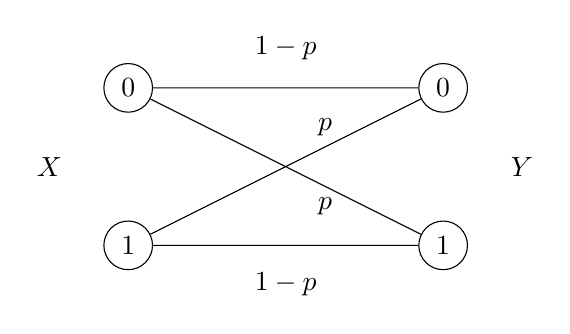
\begin{tikzpicture}
\node [draw=black,circle] (1) at(0,0) {0};
\node [draw=black,circle] (2) at(4,0) {0};
\node [draw=black,circle] (3) at(0,-2) {1};
\node [draw=black,circle] (4) at(4,-2) {1};
\draw 
(1) -- (2)
(1) -- (4)
(3) -- (2)
(3) -- (4)
;
\node (5) at(2,0.5) {$1-p$};
\node (6) at(2.5,-0.5) {$p$};
\node (7) at(2.5,-1.5) {$p$};
\node (8) at(2,-2.5) {$1-p$};
\node (9) at(-1,-1) {$X$};
\node (10) at(5,-1) {$Y$};
\end{tikzpicture}
}
\end{figure}

که در آن، پیکان ها احتمالات گذار را از متغیر تصادفی $X$ به متغیر تصادفی $Y$ نشان می دهند؛ به طور مثال
$
\Pr\{Y=0|X=1\}=p
$.

الف) اگر 
$
\Pr\{X=0\}=q
$
 که 
$
0\le q\le 1
$
، در اینصورت توزیع توام $X$ و $Y$ را محاسبه کنید.

ب) احتمال خطا (
$
\Pr\{X\ne Y\}
$
)
 را محاسبه کنید. اگر مقدار $p$ ثابت باشد، آیا احتمال خطا بر حسب $q$ نقطه‌ی بهینه دارد؟ اگر دارد آنرا بیابید و در غیر این صورت، علت را بیان کنید.

\Q
اگر توزیع تجمعی یک متغیر تصادفی ترکیبی به صورت 
$$
F(x)=\begin{cases}
0&,\quad x<0\\
{x+2\over 4}&,\quad 0\le x<1\\
1&,\quad x\ge 1
\end{cases}
$$
باشد، چگالی احتمال متغیر تصادفی 
$
X|(X\ne 0\text{\rl{ یا }}X\ne 1)
$
 را به دست آورید.


\Q
اگر برای متغیرهای تصادفی $X$ و $Y$، چگالی احتمال زیر را داشته باشیم
$$
f_{XY}(x,y)=\begin{cases}e^{-x(y+1)^2}&,\quad x,y>0\\
0&,\quad \text{\rl{در غیر این صورت}}\end{cases}
$$
در این صورت توزیع $X|Y=y$ را به دست آورید.

\Q
فرض کنید متغیر تصادفی $X$، نتیجه پرتاب یک تاس سالم باشد. سپس با توجه به رخداد 
$X$
، متغیر تصادفی پیوسته‌ی
$Y$
را به صورت شرطی با چگالی احتمال زیر تعریف می‌کنیم:
\eqn{
f_{Y|X}(x,y)=\begin{cases}
{1\over x}&,\quad 0<y<x\\
0&,\quad \text{سایر جاها}
\end{cases}
}

الف) احتمال 
$\Pr\{Y\ge 3\}$
را بیابید.

ب) چگالی احتمال 
$f_Y(y)$
را به دست آورید.

پ) مقادیر 
$\mathbb{E}\{Y\}$
و
$\text{var}(Y)$
را از روی چگالی احتمال $Y$ محاسبه کنید.



\Q
برای چگالی احتمال زیر، مقادیر
$
\mathbb{E}\{X|X>1\}
$
و
$
\sigma_X^2(X|X>1)
$
و چگالی های احتمال شرطی
$
f(x|X\ne 1)
$
و
$
f(x|X<\frac{1}{2})
$
 را محاسبه کنید.
$$
f_X(x)=\begin{cases}
3x(1-x)&,\quad 0<x<1\\
\frac{1}{2}\delta(x-1)&,\quad x=1\\
0&,\quad \text{سایر جاها}
\end{cases}
$$

\Q
چگالی احتمال توأم زیر برای دو متغیر تصادفی $X$ و $Y$ داده شده است:
$$
f_{X,Y}(x,y)=\begin{cases}
\frac{1}{\pi}&,\quad x^2+y^2\le 1\\
0&,\quad \text{سایر جاها}
\end{cases}
$$

الف) چگالی احتمال شرطی
$
f_{\max\{X,Y\}}(u|X\le \frac{1}{2})
$
را بیابید (ابتدا 
$
\Pr\{\max\{X,Y\}\le u|X\le \frac{1}{2}\}
$
را محاسبه کنید).

ب) مقدار 
$
\mathbb{E}\{\sqrt{X^2+Y^2}|X+Y\le 1\}
$
را بیابید.

\Q
اطلاعات زیر در مورد دو متغیر تصادفی $X$ و $Y$ داده شده است:
\eqn{
&\Pr\{X=-1\}=\Pr\{X=1\}=\frac{1}{2}
\\&
f_Y(y|X=x)=\frac{a}{2}\exp(-a|x-y|)
}
که $a$، عدد ثابت مثبتی است.

الف) احتمال های
$
\Pr\{Y\le 0|X=1\}
$
و
$
\Pr\{Y\ge 0|X=-1\}
$
را بیابید. با افزایش $a$، مقادیر احتمالهای فوق چه تغییر می‌کنند؟

ب) نتیجه‌ی قسمت الف را با دیدگاه احتمال خطا توجیه کنید.


%%%%%%%%%%%%%%%%%%%%%%%%%%%%%%%%%%%%%%
%%%%%%%%%%%%%%%%%%%%%%%%%%%%%%%%%%%%%%
%%%%%%%%%%%%%%%%%%%%%%%%%%%%%%%%%%%%%%
%%%%%%%%%%%%%%%%%%%%%%%%%%%%%%%%%%%%%%
%%%%%%%%%%%%%%%%%%%%%%%%%%%%%%%%%%%%%%

\chapter{دنباله‌ی متغیرهای تصادفی}

\Q
(قدم زدن تصادفی) فردی از نقطه‌ی صفر روی محور اعداد حقیقی با احتمال $p$ یک متر به سمت راست و با احتمال $1-p$ یک متر به سمت چپ می  رود. اگر این فرد این نوع قدم زدن را $n$ بار و هربار از روی نقطه ای که روی آن ایستاده تکرار کند، با چه احتمالی پس از $k$ بار قدم زدن به مبدا باز می گردد؟

\Q
فرض کنید دنباله‌ی متغیرهای تصادفی 
$\{X_n\}$،
از توزیع یکنواخت بین 
$-\frac{1}{2}$
و
$\frac{1}{2}$
به طور مستقل پیروی می‌کند. به کمک قضیه‌ی حد مرکزی، توزیع متغیر تصادفی $Y$ و میانگین و واریانس آن را به دست آورید؛ اگر 
$$Y=\lim_{n\to \infty} {X_1+X_2+\cdots +X_n\over \sqrt n}.$$

\Q
الف) تابع مولد گشتاور متغیر تصادفی پواسون با پارامتر $\lambda$  را به دست آورید.

ب) اگر دنباله‌ی متغیرهای تصادفی مستقل $\{X_n\}$، از نوع پواسون با پارامتر $\lambda$ باشد، نشان دهید متغیر تصادفی 
$$
Y=\sum_{i=1}^NX_i
,
$$
دارای توزیع پواسون با پارامتر $N\lambda$ است.

پ) نشان دهید اگر دنباله‌ی متغیرهای تصادفی مستقل $\{X_n\}$، برنولی با پارامتر $p$ و $N$ از نوع پواسون با پارامتر $\lambda$ باشد، متغیر تصادفی
$Y=\sum_{n=0}^{N-1} X_n$
 دارای توزیع پواسون با پارامتر $\lambda p$ است.



\Q
تحقیق کنید هر یک از دنباله‌ی متغیرهای تصادفی زیر، با چه مفهومی به یک متغیر تصادفی میل می‌کنند. برای هر یک دلیل بیاورید.

الف) 
$
X_n=X+{1\over n}
$
 که $X$، یک متغیر تصادفی یکنواخت در بازه‌ی $[0,1]$ است.

ب) متغیر تصادفی نمایی با پارامتر ${n+1\over n}$

پ) متوسط تعداد شیرها در $n$ بار پرتاب مستقل یک سکه‌ی سالم

\chapter{شبیه سازی ها}

\Q
سکه‌ی سالمی را (که احتمال پشت و رو برابر $1\over 2$ است) به تعداد n بار پرتاب می کنیم.

الف) منحنی تعداد دفعات رو آمدن سکه را به تعداد کل دفعات پرتاب سکه بر حسب $n$ به ازای $1\le n\le 100$ رسم کنید.

ب) رفتار این نمودار را با افزایش $n$ توصیف کرده و بیان کنید به چه عددی همگرا می شود. مشاهدات خود را توضیح دهید.

پ) همین نمودار را برای سکه غیر سالم که احتمال رو آمدن آن
$
{2\over 3}
$
است،  رسم کرده و بیان کنید به چه عددی همگرا می‌گردد. مشاهدات خود را توضیح دهید.

\textbf{
راهنمایی: ابتدا به کمک تابع 
randi()
در متلب، یک آرایه 
$1\times 100$
 از اعداد تصادفی 0 یا 1 بسازید (به عنوان مثال 0 را شیر و 1 را خط در نظر بگیرید). سپس هر بار، به ازای هر $n$ که
$1\le n \le 100$
، 
میانگین
$n$
 مقدار اول آرایه فوق را حساب کرده و آرایه‌ی $1\times 100$ جدید بسازید. آرایه‌ی جدید، پاسخ مسئله است که باید بر حسب $n$ از 1 تا 100 رسم گردد.
}



\Q
سکه ای با احتمال $p$ رو و با احتمال $1-p$ پشت می آید. آزمایشی را در نظر بگیرید که در آن، این سکه 100 بار پرتاب شده و نسبت تعداد رو آمدن ها به تعداد کل پرتاب ها (=100) به عنوان نتیجه آزمایش در نظر گرفته می شود.

اگر آزمایش فوق را $m$ بار تکرار کرده و نتیجه این $m$ آزمایش را در یک آرایه‌ی 
$
1\times m
$
 ذخیره کنیم،

الف) با فرض 
$
p=0.5
$
و
$
m=100
$
، این آرایه را رسم کنید (مشابه بند الف سوال 1). سپس به کمک قضیه دموآو-لاپلاس، منحنی گوسی را به عنوان تقریبی از توزیع دو جمله ای به همراه نمودار قبل رسم نموده و مشاهدات خود را توضیح دهید.

ب) بند الف را به ازای $m=1000$ تکرار کنید. چه تفاوتی مشاهده می شود؟

پ) بند الف را یک بار برای حالت 
$
p=0.2
$
و
$
m=1000
$
و بار دیگر برای حالت 
$
p=0.1
$
و
$
m=1000
$
شبیه سازی کنید و مشاهدات خود را توصیف کنید. چه تفاوتی با بند های پیشین مشاهده می شود؟

(یادآوری: توزیع دوجمله ای با پارامترهای $n$ و $p$ را می توان به صورت زیر با منحنی گوسی تقریب زد:
$$
\binom{n}{k}p^kq^{n-k}\approx {1\over\sqrt{2\pi npq}}e^{-{(k-np)^2\over 2npq}}
$$
که 
$
q=1-p
$.
)

\Q
سوال 1) (تعبیر تجربی چگالی احتمال) می دانید که تابع چگالی احتمال دارای شهود تجربی است؛ به این معنا که مقدار چگالی احتمال در هر نقطه از دامنه‌ی متغیر تصادفی، نشان دهنده‌ی وزن احتمالاتی آن نقطه است. برای به تصویر کشیدن این شهود، متغیر تصادفی گوسی با میانگین صفر و واریانس 1 را در نظر بگیرید. تابع
\texttt{
randn()
}
در متلب، تحققی از چنین متغیر تصادفی ای را برآورده می کند. به کمک این تابع، 100000 تحقق مستقل از این متغیر تصادفی را تولید کرده و به کمک دستور 
\texttt{
histogram()
}
آرایه‌ی 100000 تایی را رسم کنید. سپس با حفظ این نمودار، نمودار منحنی گوسی با میانگین صفر و واریانس 1 را رسم کرده و دو نمودار را با هم مقایسه کنید. مشاهدات خود را توضیح دهید.

نکته مهم!

پارامتر 
\texttt{
`Normalization'
}
را روی مقدار 
\texttt{
`pdf'
}
تنظیم کنید. برای این کار، دستور 
\texttt{
histogram()
}
را به صورت 
\texttt{
histogram(.....,'Normalization','pdf')
}
استفاده کنید.


\Q
در مبحث توابعی از یک متغیر تصادفی آموختید که اگر متغیر تصادفی $X$ دارای چگالی احتمال  مشخص باشد، آنگاه می توان چگالی احتمال  متغیر تصادفی $Y=g(X)$ را با تنظیم تابع $g(\cdot)$ روی هر تابع دلخواهی تنظیم کرد. ثابت می‌شود که اگر $X$ متغیر تصادفی یکنواخت در بازه‌ی $[0,1]$ باشد، متغیر تصادفی 
$
Y=-\ln (1-X)
$
دارای توزیع نمایی با پارامتر $\lambda=1$ و توزیع 
$
f_Y(y)=e^{-y}
$
است. برای اثبات این امر،

الف) 100000 تحقق از متغیر تصادفی یکنواخت در بازه‌ی $[0,1]$ را به کمک دستور 
\texttt{rand()}
تولید کرده و هیستوگرام آن را رسم کنید. اسم بردار 100000 تایی را $X$ بگذارید.

ب) از روی بردار $X$، بردار 100000 تایی $Y=-\ln(1-x)$ را محاسبه کرده و هیستوگرام آن را رسم کنید. سپس چگالی احتمال متغیر تصادفی نمایی با پارامتر $\lambda=1$ را به همراه این هیستوگرام در یک نمودار نشان دهید. رابطه‌ی بین هیستوگرام و چگالی احتمال  توزیع نمایی را توجیه کنید.

برای رسم دو نمودار در یک شکل، از دستور 
\texttt{\lr{hold on}}
استفاده کنید.

\Q
در این شبیه سازی، قصد داریم پرتاب سکه را با جزئیات بیشتر مطالعه کنیم. می‌دانیم در 
$
n
$
بار پرتاب سکه‌ی سالم، احتمال 
$
k
$
بار رو آمدن برابر است با
$$
\binom{n}{k}(\frac{1}{2})^n.
$$
جهت تجربه‌ی عملی فرمول اخیر، آزمایشی را که در آن سکه
$
1000
$
بار پرتاب می‌شود،
$
1000
$
بار تکرار می‌کنیم (مشابه اینکه سکه ای را 1000000 بار پرتاب کرده و هر 1000 نتیجه‌ی پشت سر هم را خوشه‌بندی کنیم).

گامها:

گام 1) به کمک یک حلقه‌ی \lr{for}،
1000 عدد تصادفی 0 یا 1 تولید کرده و تعداد دفعاتی را که این رشته‌ی 1000تایی برابر 1 می‌شود (سکه رو می‌آید) را حساب کنید.

گام 2) گام1 را 1000 بار تکرار کرده و هر بار نتیجه را در یک آرایه‌ی 1000تایی ذخیره کنید.

گام 3) هیستوگرام نتایج را رسم نموده و آن را توجیه کنید (تعداد \lr{bin}های هیستوگرام را برابر $40$ قرار دهید).

سوال 2)

الف) می‌دانیم که چگالی احتمال یک متغیر تصادفی، میانگین تجربی تعداد دفعات رخداد مقادیر آن متغیر تصادفی را نشان می‌دهد؛ به طور مثال در توزیع یکنواخت در بازه‌ی $[0,1]$، تمام اعداد این بازه، دارای میانگین تجربی یکسان رخداد هستند. جهت تحقیق این امر، 10000 تحقق از توزیع یکنواخت در بازه‌ی $[0,1]$ را تولید کرده و هیستوگرام آن را رسم کنید. نتیجه را توجیه کنید.

ب) می‌دانیم که اگر 
$
X
$
از توزیع یکنواخت در بازه‌ی 
$
[0,1]
$
پیروی کند، 
$
Y=-\ln X
$
از توزیع نمایی با پارامتر 
$
\lambda=1
$
پیروی می‌کند و چگالی احتمال آن به صورت زیر است:
$$
f_Y(y)=\begin{cases}
e^{-y}&,\quad y>0\\
0&,\quad y\le0\\
\end{cases}.
$$
به کمک دستور هیستوگرام، 10000 تحقق از توزیع یکنواخت در بازه‌ی 
$
[0,1]
$
تولید کرده و در آرایه‌ای به نام
$
X
$
ذخیره کنید. سپس آرایه‌ی
$
Y
$
را از روی آرایه‌ی
$
X
$
به صورت
$
Y=-\ln X
$
بسازید. سپس هیستوگرام $Y$ را با تعداد \lr{bin} برابر 100 رسم کنید. جهت مشاهده‌ی رفتار چگالی احتمال، تابع
$
e^{-y}
$
را در بازه‌ی 
$
(0,10)
$
روی همان نمودار هیستوگرام رسم شده بکشید و نتیجه را توجیه کنید.

(
فرض کنید میخواهید هیستوگرام آرایه‌ی $x$ را رسم کنید. جهت رسم هیستوگرام در این سوال، از دستورهای زیر استفاده کنید:

%متلب:
%\begin{latin}
%\begin{minted}{matlab}
%histogram(x,'Normalization','pdf')
%\end{minted}
%\end{latin}
%پایتون:
%\begin{latin}
%\begin{minted}{python}
%hist(x,density='pdf')
%\end{minted}
%\end{latin}

)

%\chapter{پاسخ سوالات}
%
%\QA
%از اصل سوم احتمال، برای هر دو مجموعه‌ی ناسازگار 
%$A$
%و
%$B$
%داریم
%$$P(A\cup B)=P(A)+P(B).$$
%از آنجا که 
%$A$
%و
%$A'$
%طبق تعریف ناسازگارند، بنابراین
%$$P(A\cup A')=P(A)+P(A').$$
%از طرفی طبق تعریف،
%$$A\cup A'=S$$
%که $S$ فضای نمونه است. در نتیجه
%$$P(A)+P(A')=1.$$
%بر اساس اصل اول احتمال، احتمال هر مجموعه مقداری نامنفی است؛ در نتیجه
%$$P(A)=1-P(A')\le 1$$
%و اثبات کامل است
%$\blacksquare$



\end{document}